\documentclass[11pt]{article}

% if you need to pass options to natbib, use, e.g.:
%\PassOptionsToPackage{numbers}{natbib}
\usepackage[colorlinks,linkcolor=blue,filecolor=blue,citecolor=magenta,urlcolor=blue]{hyperref}
\usepackage{bm,amsmath,amsthm,amssymb,multicol,algorithmic,algorithm,enumitem,graphicx,subfigure}
\usepackage{xargs}
\usepackage{stmaryrd}
\usepackage{natbib}
% \usepackage[english]{babel}

% ready for submission
\usepackage{neurips_2021}
\def\M{\mathcal{M}}
\def\A{\mathcal{A}}
\def\Z{\mathcal{Z}}
\def\S{\mathcal{S}}
\def\D{\mathcal{D}}
\def\R{\mathcal{R}}
\def\P{\mathcal{P}}
\def\K{\mathcal{K}}
\def\E{\mathbb{E}}
\def\F{\mathfrak{F}}
\def\l{\boldsymbol{\ell}}

\newtheorem{Fact}{Fact}
\newtheorem{Lemma}{Lemma}
\newtheorem{Prop}{Proposition}
\newtheorem{Theorem}{Theorem} 
\newtheorem{Def}{Definition}
\newtheorem{Corollary}{Corollary}
\newtheorem{Conjecture}{Conjecture}
\newtheorem{Property}{Property}
\newtheorem{Observation}{Observation}
\newtheorem{Exa}{Example}
\newtheorem{assumption}{H\!\!}
\newtheorem{Remark}{Remark}
\newtheorem*{Lemma*}{Lemma}
\newtheorem*{Theorem*}{Theorem}
\newtheorem*{Corollary*}{Corollary}
 
\newcommand{\eqsp}{\;}
\newcommand{\beq}{\begin{equation}}
\newcommand{\eeq}{\end{equation}}
\newcommand{\eqdef}{\mathrel{\mathop:}=}
\def\EE{\mathbb{E}}
\newcommand{\norm}[1]{\left\Vert #1 \right\Vert}
\newcommand{\pscal}[2]{\left\langle#1\,|\,#2 \right\rangle}
\def\major{\mathsf{M}}
\def\rset{\ensuremath{\mathbb{R}}}

\begin{document}
\title{Distributed Adaptive Learning with Gradient Compression}

\author{
Xiaoyun Li \\
  Cognitive And Computing Lab\\
  Baidu Research\\
  Beijing, USA \\
  \texttt{xiaoyun@baidu.com} 
   \And
  Belhal Karimi \\
  Cognitive And Computing Lab\\
  Baidu Research\\
  Beijing, China \\
  \texttt{v_karimibelhal@baidu.com} 
   \And
  Ping Li \\
  Cognitive And Computing Lab\\
  Baidu Research\\
  Beijing, China \\
  \texttt{liping@baidu.com} \\
}

\date{\today}

\maketitle

\begin{abstract}
This paper presents a new algorithm -- the Sparsified AMSGrad algorithm (\algo) -- for tackling single-machine and distributed supervised learning.
Unlike prior works which rely on full gradient communication between the workers and the parameter-server, we design a distributed adaptive optimization method with gradient compression coupled with an error-feedback to alleviate the bias introduced by the compression.
While the former allows us to only transmit fewer bits of gradient vectors to the server, we show that using the latter, which correct for the bias, \algo\ reaches a stationary point in $\mathcal{O}(1/ \sqrt{T})$ iterations, matching that of state-of-the-art single-machine and distributed methods, without any error-feedback.
We illustrate our theoretical results by showing the effectiveness of our method both under the single-machine and distributed settings on various benchmark datasets.
%In this paper, we present a novel optimization algorithm for single-machine and distributed learning, based on sparsification and error feedback techniques to lighten the communications between a central server and distributed workers.
%The method we introduce builds on the adaptivity of the AMSGrad method for nonconvex optimization, and includes a TopK operation to alleviate any communication bottleneck between a large amount of devices and a central computing server, combined with a correction of the natural bias induced by the latter compression operator.
%Despite the sparsity induced by our algorithm, we show that \algo reaches a stationary point in $\mathcal{O}(1/ \sqrt{T})$ iterations, matching that of state-of-the-art single-machine methods.
\end{abstract}

\section{Introduction}\label{sec:introduction}

Deep neural network has achieved the state-of-the-art learning performance on numerous AI applications, e.g., computer vision~\cite{Proc:GAN_NIPS14,Proc:Resnet_CVPR16,CV_review18}, Natural Language Processing~\cite{Proc:Graves_ICASSP13,NLP_review18,sentiment_review18}, Reinforcement Learning~\cite{Arxiv:MnihKSGAWR13,AlphaGo_17} and recommendation systems~\cite{Proc:Covington_2016,Article:Wei_2017}. With the increasing size of both data and deep networks, standard single machine training confronts with at least two major challenges:
\begin{itemize}
    \item Due to the limited computing power of a single machine, it would take a long time to process the massive number of data samples---training would be slow.
  
    \item In many practical scenarios, data are typically stored in multiple servers, possibly at different locations, due to the storage constraints (massive user behavior data, Internet images, etc.) or privacy reasons~\cite{Proc:Chang18}. Transmitting data might be costly.
\end{itemize}
\textit{Distributed learning} framework~\cite{Proc:Dean_NIPS12} has been a common training strategy to tackle the above two issues. For example, in centralized distributed stochastic gradient descent (SGD) protocol, data are located at $n$ local nodes, at which the gradients of the model are computed in parallel. In each iteration, a central server aggregates the local gradients, updates the global model, and transmits back the updated model to the local nodes for subsequent gradient computation. As we can see, this setting naturally solves aforementioned issues: 1) We use $n$ computing nodes to train the model, so the time per training epoch can be largely reduced; 2) There is no need to transmit the local data to central server. Besides, distributed training also provides stronger error tolerance since the training process could continue even one local machine breaks down. As a result of these advantages, there has been a surge of study and applications on distributed systems~\cite{boyd2011distributed,nedic2009distributed,duchi2011dual,Arxiv:Goyal17,hong2017prox,lu2019gnsd,koloskova2019decentralized}.

Among many optimization strategies, SGD is still the most popular prototype in distributed training for its simplicity and effectiveness~\cite{chilimbi2014project,Proc:Agrawal_NIPS19,mikami2018massively}. Yet, when the deep learning model is very large, the communication between local nodes and central server could be expensive. Burdensome gradient transmission would slow down the whole training system, or even be impossible because of the limited bandwidth in some applications. Thus, reducing the communication cost in distributed SGD has become an active topic, and an important ingredient of large-scale distributed systems (e.g.~\cite{Proc:Seide14}). Solutions based on quantization, sparsification and other compression techniques of the local gradients are proposed, e.g.,~\cite{alistarh2017qsgd,wen2017terngrad,wangni2018gradient,stich2018sparsified,aji2017sparse,bernstein2018signsgd,de2017understanding,yang2019swalp,Proc:Ivkin_NIPS19}. As one would expect, in most approaches, there exists a trade-off between compression and learning performance. In general, larger bias and variance of the compressed gradients usually bring more significant performance downgrade in terms of convergence~\cite{stich2018sparsified,ajalloeian2020analysis}. Interestingly, studies (e.g.,~\cite{karimireddy2019error}) show that the technique of \textit{error feedback} is able to remedy the issue of such biased compressors, achieving same convergence rate as full-gradient SGD.


On the other hand, in recent years, adaptive optimization algorithms (e.g. AdaGrad~\cite{Duchi10-adagrad}, Adam~\cite{kingma2014adam} and AMSGrad~\cite{reddi2019convergence}) have become popular because of their superior empirical performance. These methods use different implicit learning rates for different coordinates that keep changing adaptively throughout the training process, based on the learning trajectory. In many learning problems, adaptive methods have been shown to converge faster than SGD, sometimes with better generalization as well. However, the body of literature that combines adaptive methods with distributed training is still very limited. In this papar, we propose a distributed optimization algorithm with AMSGrad as the backbone, along with Top-$k$ sparsification to reduce the communication cost.

\subsection{Our contributions}

We develop a simple optimization leveraging the adaptivity of AMSGrad, and the computational virtue of TopK sparsification, for tackling a large finite-sum of nonconvex objective functions.

Our technique is shown to be both theoretically and empirically effective under \emph{the classical centralized setting} and \emph{the distributed setting}.

In this contribution, 
\begin{itemize}
\item We derive a sparsified AMSGrad with error feedback, called \algo, with a single machine and provide its decentralized counter part.
\item We provide a non-asymptotic convergence rate under each setting,
\item We highlight the effectiveness of both methods through several numerical experiments
\end{itemize}


\section{Related Work}\label{sec:related}

\subsection{Distributed SGD with compressed gradients}

\paragraph{Quantization.} As we mentioned before, SGD is the most commonly adopted optimization method in distributed training of deep neural nets. To reduce the expensive communication in large-scale distributed systems, extensive works have considered various compression techniques applied to the gradient transaction procedure. The first strategy is quantization. \cite{Proc:8-bit_ICLR16} condenses 32-bit floating numbers into 8-bits when representing the gradients. \cite{Proc:Seide14,bernstein2018signsgd,karimireddy2019error,Proc:Bernstein_ICLR19} use the extreme 1-bit information (sign) of the gradients, combined with tricks like momentum, majority vote and memory. Other quantization-based methods include QSGD~\cite{alistarh2017qsgd,Proc:Wu_ICML18,Proc:Zhang_ICML17} and LPC-SVRG~\cite{Proc:Yu_AISTATS19}, leveraging unbiased stochastic quantization. The saving in communication of quantization methods is moderate: for example, 8-bit quantization reduces the cost to 25\% (compared with 32-bit full-precision). Even in the extreme 1-bit case, the largest compression ratio is around $1/32\approx 3.1\%$. 

\paragraph{Sparsification.} Gradient sparsification is another popular solution which may provide higher compression rate. Instead of commuting the full gradient, each local worker only passes a few coordinates to the central server and zeros out the others. Thus, we can more freely choose higher compression ratio (e.g., 1\%, 0.1\%), still achieving impressive performance in many applications~\cite{Proc:Lin_ICLR18}. Stochastic sparsification methods, including uniform sampling and magnitude based sampling~\cite{wangni2018gradient}, select coordinates based on some sampling probability yielding unbiased gradient compressors. Deterministic methods are simpler, e.g., Random-$k$, Top-$k$~\cite{stich2018sparsified,shi2019convergence} (selecting $k$ elements with largest magnitude), Deep Gradient Compression~\cite{Proc:Lin_ICLR18}, but usually lead to biased gradient estimation. In~\cite{Proc:Ivkin_NIPS19}, the central server identifies heavy-hitters from the count-sketch~\cite{Proc:Charikar_ICALP02} of the local gradients, which can be regarded as a noisy variant of Top-$k$ strategy. More applications and analysis of compressed distributed SGD can be found in~\cite{jiang2018linear,Proc:Shen_ICML18,alistarh2018convergence,Proc:Basu_NIPS19,Proc:Jiang_SIGMOD18}, among others.

\paragraph{Error Feedback.} Biased gradient estimation, which is a consequence of many aforementioned methods (e.g., signSGD, Top-$k$), undermines the model training, both theoretically and empirically, with slower convergence and worse generalization~\cite{ajalloeian2020analysis,Arxiv:Beznosikov20}. The technique of \textit{error feedback} is able to ``correct for the bias'' and fix the problems. In this procedure, the difference between the true stochastic gradient and the compressed one is accumulated locally, which is then added back to the local gradients in later iterations. \cite{stich2018sparsified,karimireddy2019error} prove the $\mathcal O(\frac{1}{T})$ and $\mathcal O(\frac{1}{\sqrt T})$ convergence rate of EF-SGD in strongly convex and non-convex setting respectively, matching the rates of vanilla SGD~\cite{nemirovski2009robust,ghadimi2013stochastic}.


\subsection{Adaptive optimization}

In each SGD update, all the gradient coordinates share a same learning rate, either constant or decreasing over iterations. Adaptive optimization methods cast different learning rate on each dimension. AdaGrad~\cite{Duchi10-adagrad} divides the gradient element-wisely by $\sqrt{\sum_{t=1}^T g_{t}^2}\in \mathbb R^d$, where $g_{t}\in \mathbb R^d$ is the gradient vector at time $t$ and $d$ is the model dimensionality. Thus, it intrinsically assigns different learning rates to different coordinates throughout the training---elements with smaller previous gradient magnitude tend to move a larger step. AdaGrad has been shown to perform well especially under some sparsity structure. AdaDelta~\cite{Proc:adadelta} and Adam~\cite{kingma2014adam} introduce momentum and moving average of second moment estimation into AdaGrad which lead to better performance. AMSGrad~\cite{reddi2019convergence} fixes the potential convergence issue of Adam, which will serve as the prototype in this paper. We present the psudocode in Algorithm . In general, adaptive optimization methods are easier to tune in practice, and usually exhibit faster convergence than SGD. Thus, they have been widely used in training deep learning models in language and computer vision applications, e.g.,~\cite{,Arxiv:Choi_2019,Proc:LAMB_ICLR20,Arxiv:Zhang_ICLR21}. In distributed setting, the work~\cite{nazari2019dadam} proposes a decentralized system in online optimization. However, communication efficiency is not considered. The recent work~\cite{chen2020quantized} is the most relevant to our paper. Yet, their method is based on Adam, and requires every local node to store a local estimation of first and second moment, thus being less efficient. We will present more detailed comparison in Section~\ref{sec:main}.


\section{Communication-Efficient Adaptive Optimization}\label{sec:main}

\subsection{Gradient Compressors}

In this paper, we mainly consider deterministic $q$-deviate compressors defined as below.

\begin{assumption}\label{ass:quant} We say a compressor $\mathcal C:\mathbb R^d\mapsto \mathbb R^d$ is $q$-deviate if for $\forall x\in\mathbb R^d$, $\exists$ $0\leq q < 1$ such that $\norm{\mathcal C(x)-x} \leq q \norm{x}$.
\end{assumption}
Note that, smaller $q$ indicates better approximation of the true gradient, and $q=0$ implies no compression, i.e.~$\mathcal C(x)=x$. We give two popular and highly efficient $q$-deviate compressors that will be compared in this paper.

\begin{definition}[Top-$k$]\label{def:topk}
For $x\in\mathbb R^d$, denote $\mathcal S$ as the size-$k$ set of $i\in[d]$ with largest $k$ magnitude $|x_i|$. The \textbf{Top-$k$} compressor is defined as $\mathcal C(x)_i=x_i$, if $i\in\mathcal S$; $\mathcal C(x)_i=0$ otherwise.
\end{definition}

\begin{definition}[SIGN]\label{def:sign}
For $x\in\mathbb R^d$, define the \textbf{SIGN} compressor as $\mathcal C(x)=sign(x)\times \frac{1}{d}\sum_{i=1}^d |x_i|$. 
\end{definition}
\begin{Remark}
Here the scalar, mean magnitude, multiplied to $sign(x)$ ensures $0\leq q<1$ as required by Assumption~\ref{ass:quant}, which can be shown by Cauchy-Schwartz inequality. In implementation, this scalar can be arbitrary since we can offset its influence by tuning the learning rate. 
\end{Remark}

Most modern machine learning tasks can be casted as a large finite-sum optimization problem written as:
\begin{equation}\label{eq:opt}
\min \limits_{\theta \in \Theta} \frac{1}{n} \sum_{i=1}^n f_i(\theta)
\end{equation}
where $n$ denotes the number of workers, $f_i$ represents the average loss for worker $i$ and $\theta$ the global model parameter taking value in $\Theta$, a subset of $\mathbb{R}^d$.



Some related work:


\citep{karimireddy2019error} develops variant of signSGD (as a biased compression schemes) for distributed optimization. Contributions are mainly on this error feedback variant.
In \citep{shi2019convergence}, the authors provide theoretical results on the convergence of sparse Gradient SGD for distributed optimization (we want that for AMS here).
\citep{stich2018sparsified} develops a variant of distributed SGD with sparse gradients too. Contributions include a memory term used while compressing the gradient (using top k for instance). Speeding up the convergence in $\frac{1}{T^3}$.
% \url{https://arxiv.org/pdf/1901.09847.pdf}
% \url{https://pdfs.semanticscholar.org/8728/dee89906022c1d4f5c1de1233c3f65ab92f2.pdf?_ga=2.152244026.2027005181.1606271153-15127215.1603945483}
% \url{https://proceedings.neurips.cc/paper/2018/file/b440509a0106086a67bc2ea9df0a1dab-Paper.pdf}

Consider standard synchronous distributed optimization setting. AMSGrad is used as the prototype, and the local workers is only in charge of gradient computation.


\subsection{\algo\ with Error Feedback}




The key difference (and interesting part) of our TopK AMSGrad compared with the following arxiv paper ``Quantized Adam''\url{https://arxiv.org/pdf/2004.14180.pdf} is that, in our model only gradients are transmitted. In ``QAdam'', each local worker keeps a local copy of moment estimator $m$ and $v$, and compresses and transmits $m/v$ as a whole. Thus, that method is very much like the sparsified distributed SGD, except that $g$ is changed into $m/v$. In our model, the moment estimates $m$ and $v$ are computed only at the central server, with the compressed gradients instead of the full gradient. This would be the key (and difficulty) in convergence analysis.


\begin{algorithm}[H]
\caption{Distributed \algo\ with error-feedback} \label{alg:sparsams}
\begin{algorithmic}[1]

\STATE \textbf{Input}: parameter $\beta_1$, $\beta_2$, learning rate $\eta_t$. 
\STATE Initialize: central server parameter $\theta_{1} \in \Theta \subseteq \mathbb R^d$; $e_{1,i}=0$ the error accumulator for each worker; sparsity parameter $k$; $n$ local workers; $m_0=0$, $v_0=0$, $\hat v_0=0$

\FOR{$t=1$ to $T$}

\STATE\textbf{parallel for worker $i \in [n]$ do}:
\STATE\quad  Receive model parameter $\theta_{t}$ from central server
\STATE\quad  Compute stochastic gradient $g_{t,i}$ at $\theta_t$
\STATE\quad  Compute $\tilde g_{t,i}=TopK(g_{t,i}+e_{t,i},k)$ \label{line:topk} 
\STATE\quad  Update the error $e_{t+1,i}=e_{t,i}+g_{t,i}-\tilde g_{t,i}$
\STATE\quad  Send $\tilde g_{t,i}$ back to central server
\STATE \textbf{end parallel}

\STATE \textbf{Central server do:}
\STATE $\bar g_{t}=\frac{1}{n}\sum_{i=1}^n \tilde g_{t,i}$
\STATE $m_t=\beta_1 m_{t-1}+(1-\beta_1)\bar g_t$
\STATE $v_t=\beta_2 v_{t-1}+(1-\beta_2)\bar g_t^2$
\STATE $\hat v_t=\max(v_t,\hat v_{t-1})$ \label{line:v}
\STATE Update the global model $\theta_{t+1}=\theta_{t}-\eta_t\frac{m_t}{\sqrt{\hat v_t+\epsilon}}$

\ENDFOR
\end{algorithmic}
\end{algorithm}


\section{Non-Asymptotic Convergence Analysis for the Single Machine and Decentralized settings}

Several mild assumptions to make: Nonconvex and smooth loss function, unbiased stochastic gradient, bounded variance of the gradient, bounded norm of the gradient, control of the distance between the true gradient and its sparse variant.

Check \citep{chen2020quantized} starting with single machine  and extending to distributed settings (several machines).


Under the distributed setting, the goal is to derive an upper bound to the second order moment of the gradient of the objective function at some iteration $T_f \in [1, T]$.


We begin by making the following assumptions.

\begin{assumption}\label{ass:smooth}(Smoothness)
For $i \in \inter$, $f_i$ is  L-smooth: $\norm{\nabla f_i (\theta) - \nabla f_i (\vartheta)} \leq L \norm{\theta-\vartheta}$.
\end{assumption}

\begin{assumption}\label{ass:boundgrad}(Unbiased and Bounded gradient \textbf{per worker})
For any iteration index $t >0$ and worker index $i \in \inter$, the stochastic gradient is unbiased and bounded from above: $\EE[g_{t,i}] = \nabla f_i(\theta_t)$ and $\norm{g_{t,i}} \leq G_i$.
\end{assumption}

\begin{assumption}\label{ass:var}(Bounded variance \textbf{per worker})
For any iteration index $t >0$ and worker index $i \in \inter$, the variance of the noisy gradient is bounded: $\EE[|g_{t,i} - \nabla f_i(\theta_t)|^2] < \sigma_i^2$.
\end{assumption}

Denote by $Q(\cdot)$ the quantization operator Line~\ref{line:topk} of Algorithm~\ref{alg:sparsams}, which takes as input a gradient vector and returns a quantized version of it, and note $\tilde{g} \eqdef Q(g)$.
Assume that



Denote for all $\theta \in \Theta$:
\begin{equation}\label{eq:obj}
f(\theta) \eqdef  \frac{1}{n} \sum_{i=1}^n f_i(\theta) \, ,
\end{equation} 
where $n$ denotes the number of workers.






\paragraph{Decentralized Workers Setting:}

The main theorem in the decentralized setting reads:

\begin{Theorem}\label{thm:mainmultiple}
Under Assumption~\ref{ass:smooth} to Assumption~\ref{ass:var}, the sequence of iterates $\{\theta_t\}_{t>0}$ output from Algorithm~\ref{alg:sparsams} satisfies:

\begin{equation}
\begin{split}
 \frac{1}{\maxiter}\sum_{t=1}^{\maxiter} \EE[\norm{\nabla f(\theta_t)}^2] \leq \frac{\EE[ f(\theta_{1}) - f(\theta_{\maxiter+1})]}{ \Delta_1 \eta_t \maxiter} + 
d\frac{ \Delta_3}{\Delta_1 \eta_t \maxiter}  + \frac{\Delta_2}{ \Delta_1\maxiter} +\frac{1-\beta_1}{\Delta_1}  \epsilon^{-\frac{1}{2}} \sqrt{(q^2+1)}\sigma^2 
\end{split}
\end{equation}


where $\{\eta_t\}_{t>0}$ is the sequence of stepsizes and:
\begin{equation}
\begin{split}
\Delta_1 & \eqdef \frac{(1-\beta_1)}{2} (\epsilon + \frac{(q^2+1)\sigma^2}{1 - \beta_2})^{-\frac{1}{2}} \quad \textrm{,} \quad \Delta_2 \eqdef q^2 + \frac{G^2 }{\epsilon 2n^2}  \overline{\beta}_1\\
\Delta_3 &\eqdef \left(\frac{L}{2} + 1+ \frac{\beta_1L}{1-\beta_1} \right) (1-\beta_2)^{-1} (1 - \frac{\beta_1^{2}}{\beta_2})^{-1}
\end{split}
\end{equation}
\end{Theorem}

We remark from this bound in Theorem~\ref{thm:mainmultiple}, that the more quantization we apply to our gradient vectors ($q \uparrow$), the larger the upper bound of the stationary condition is, \ie the slower the algorithm is. 
This is intuitive as using compressed quantities will definitely impact the algorithm speed.
We will observe in the numerical section below that a trade-off on the level of quantization $q$ can be found to achieve similar speed of convergence with less computation resources used throughout the training.


\begin{Corollary}\label{coro:mainmultiple}
Under Assumption~\ref{ass:smooth} to Assumption~\ref{ass:var},setting the stepsize as $\eta_t = L\sqrt{\frac{n}{\maxiter}}$, the sequence of iterates $\{\theta_t\}_{t>0}$ output from Algorithm~\ref{alg:sparsams} satisfies:

\begin{align*}
    \frac{1}{T}\sum_{t=1}^T \mathbb E[\|\nabla f(\theta_t)\|^2]\leq \mathcal O(\frac{1}{L\sqrt nT}+ d\frac{L}{\sqrt nT}+\frac{1}{T}),
\end{align*}
\end{Corollary}




\paragraph{Single Machine Setting:}

We first provide the formulation of our method in the single machine settings in Algorithm~\ref{alg:sparsamssingle}.
Here, the data and the computation are all performed on a single machine.

\begin{algorithm}[H]
\caption{\algo\ with error-feedback for a single machine} \label{alg:sparsamssingle}
\begin{algorithmic}[1]

\STATE \textbf{Input}: parameter $\beta_1$, $\beta_2$, learning rate $\eta_t$. 
\STATE Initialize: central server parameter $\theta_{1} \in \Theta \subseteq \mathbb R^d$; $e_{1}=0$ the error accumulator; sparsity parameter $k$; $m_0=0$, $v_0=0$, $\hat v_0=0$

\FOR{$t=1$ to $T$}
\STATE  Compute stochastic gradient $g_{t} = g_{t,i_t}$ at $\theta_t$ for randomly sampled index $i_t$\label{line:stochgrad} 
\STATE  Compute $\tilde g_{t}=TopK(g_{t}+e_{t},k)$ \label{line:topksingle} 
\STATE  Update the error $e_{t+1}=e_{t}+g_{t}-\tilde g_{t}$
\STATE $m_t=\beta_1 m_{t-1}+(1-\beta_1)\tilde g_t$
\STATE $v_t=\beta_2 v_{t-1}+(1-\beta_2)\tilde g_t^2$
\STATE $\hat v_t=\max(v_t,\hat v_{t-1})$ \label{line:vsingle}
\STATE Update the global model $\theta_{t+1}=\theta_{t}-\eta_t\frac{m_t}{\sqrt{\hat v_t+\epsilon}}$

\ENDFOR
\end{algorithmic}
\end{algorithm}


The convergence rate of the vector of parameters estimated via Algorithm~\ref{alg:sparsamssingle} is given below:
\begin{Theorem}\label{thm:mainsingle}
Under Assumption~\ref{ass:smooth} to Assumption~\ref{ass:var}, with a decreasing sequence of stepsize $\{\eta_t\}_{t>0} = \frac{1}{\sqrt{\maxiter}}$, the sequence of iterates $\{\theta_t\}_{t>0}$ output from Algorithm~\ref{alg:sparsamssingle} satisfies:
\begin{align*}
    \frac{1}{T}\sum_{t=1}^T \mathbb E[\|\nabla f(\theta_t)\|^2]\leq \mathcal O(\frac{1}{\sqrt T}+\frac{1}{T}),
\end{align*}

\end{Theorem}

matching the convergence rate of SGD with error feedback~\cite{karimireddy2019error}.


\newpage
\section{Experiments}\label{sec:experiment}
Our proposed TopK-EF with AMSGrad matches that of full AMSGrad, in distributed learning. Number of local workers is 20. Error feedback fixes the convergence issue of using solely the TopK gradient. 

\begin{figure}[H]
    \begin{center}
    \mbox{\hspace{-0.3in}
        \includegraphics[width=2.2in]{figure/mnist_cnn_test_accuracy.eps}
        \includegraphics[width=2.2in]{figure/cifar_cnn_test_accuracy.eps}
        \includegraphics[width=2.2in]{figure/cifar_lenet_test_accuracy.eps}
    }
    \end{center}
    \vspace{-0.1in}
	\caption{Test accuracy.}
	\label{fig:test accuracy}
\end{figure}



\section{Conclusion}\label{sec:conclusion}



\newpage
\bibliographystyle{plain}
\bibliography{ref}

\newpage
\appendix 


\section{Single Machine Setting}


\subsection{Intermediary Lemmas}



\begin{Lemma} \label{lemma:m_t,m_t'}
Under Assumption\ref{ass:quant} to Assumption\ref{ass:var} we have:
\begin{align*}
    &\mathbb E\|m_t'\|^2\leq C\sigma^2+C_1 \sum_{\tau=1}^t (\beta_1^2(2-\beta_1^2))^{t-\tau}\mathbb E[\|\nabla f(\theta_\tau)\|^2],\\
    &\mathbb E[\|m_t\|^2]\leq (3q^2+\frac{4q^2(6q^2+3)}{(1-q^2)^2}+1)C\sigma^2+(6q^2+3)C_1\sum_{\tau=1}^t (\beta_1^2(2-\beta_1^2))^{t-\tau}\mathbb E[\|\nabla f(\theta_\tau)\|^2],
\end{align*}
where $C_1=(1-\beta_1^2)(1+\frac{1}{4(1-\beta_1^2)})$ and $C=\frac{C_1}{1-\beta_1^2(2-\beta_1^2)}$.
\end{Lemma}

\begin{proof}
We have by Young's inequality
\begin{align*}
    \mathbb E[\|m_t'\|^2]&=\mathbb E[\|\beta_1m_{t-1}'+(1-\beta_1)g_t\|^2]\\
    &\leq (1+\rho)\beta_1^2 \mathbb E[\|m_{t-1}'\|^2]+(1+\frac{1}{\rho})(1-\beta_1)^2 \mathbb E[\|g_t\|^2].
\end{align*}
Since $\mathbb E[\|g_t\|^2]\leq \sigma^2+ \EE[\|\nabla f(\theta_t)\|^2]$, by choosing $\rho=1-\beta_1^2$, we derive
\begin{align}
    \mathbb E[\|m_t'\|^2]&\leq \beta_1^2(2-\beta_1^2)\mathbb E[\|m_{t-1}'\|^2]+(1-\beta_1)^2(1+\frac{1}{4(1-\beta_1^2)})\mathbb E[\|g_t\|^2]\\
    &\leq \frac{(1-\beta_1)^2}{1-\beta_1^2(2-\beta_1^2)}(1+\frac{1}{4(1-\beta_1^2)})\sigma^2+C_1 \sum_{\tau=1}^t (\beta_1^2(2-\beta_1^2))^{t-\tau}\mathbb E[\|\nabla f(\theta_\tau)\|^2]\\
    &\eqdef C\sigma^2+C_1 \sum_{\tau=1}^t (\beta_1^2(2-\beta_1^2))^{t-\tau}\mathbb E[\|\nabla f(\theta_\tau)\|^2],
\end{align}
due to $\beta_1<1$, $m_0'=0$ and the bounded variance assumption. Here $C_1=(1-\beta_1^2)(1+\frac{1}{4(1-\beta_1^2)})$ and $C=\frac{C_1}{1-\beta_1^2(2-\beta_1^2)}$.

For $m_t$ which consists of the compressed stochastic gradients, first note that
\begin{align*}
    \mathbb E[\|\tilde g_t\|^2]&=\mathbb E[\|\mathcal C(g_t+e_t)-(g_t+e_t)+g_t+e_t-\nabla f(\theta_t)+\nabla f(\theta_t)\|^2]\\
    &\leq \sigma^2+3\mathbb E[q^2\|g_t+e_t-\nabla f(\theta_t)+\nabla f(\theta_t)\|^2+\|e_t\|^2+\|\nabla f(\theta_t)\|^2]\\
    &\leq (3 q^2+1)\sigma^2+(6q^2+3)\mathbb E[\|e_t\|^2+\|\nabla f(\theta_t)\|^2]\\
    &\leq (3q^2+\frac{4q^2(6q^2+3)}{(1-q^2)^2}+1)\sigma^2+(6q^2+3)\mathbb E[\|\nabla f(\theta_t)\|^2],
\end{align*}
where the first inequality is because of Assumption~\ref{ass:quant} and that the stochastic error $(g_t-\nabla f(\theta_t))$ is mean-zero and independent of other terms. The bound on $\|e_t\|^2$ in the last inequality is due to Lemma 3 of~\cite{karimireddy2019error}. Then by similar induction we can obtain
\begin{align*}
    \mathbb E[\|m_t\|^2]&\leq (3q^2+\frac{4q^2(6q^2+3)}{(1-q^2)^2}+1)C\sigma^2+(6q^2+3)C_1\sum_{\tau=1}^t (\beta_1^2(2-\beta_1^2))^{t-\tau}\mathbb E[\|\nabla f(\theta_\tau)\|^2].
\end{align*}

\begin{Lemma} \label{bound:a_t}
Suppose $\gamma=\beta_1/\beta_2<1$. Then, for $\forall t$,
\begin{align*}
    \|a_t\|^2\eqdef \|\frac{m_t}{\sqrt{\hat v_t+\epsilon}} \|^2\leq \frac{(1-\beta_1)d}{(1-\beta_2)(1-\gamma)}.
\end{align*}

\end{Lemma}

\begin{proof}
We have
\begin{align*}
    \|\frac{m_t}{\sqrt{\hat v_t+\epsilon}} \|^2&=\sum_{i=1}^d \frac{m_{t,i}^2}{\hat v_{t,i}+\epsilon}\\
    &\leq \frac{(1-\beta_1)^2}{1-\beta_2}\sum_{i=1}^d \frac{(\sum_{\tau=1}^t \beta_1^{t-\tau} \tilde g_{\tau,i})^2}{\sum_{\tau=1}^t \beta_2^{t-\tau} \tilde g_{\tau,i}^2}\\
    &\overset{(a)}{\leq} \frac{(1-\beta_1)^2}{1-\beta_2}\sum_{i=1}^d \frac{(\sum_{\tau=1}^t \beta_1^{t-\tau})(\sum_{\tau=1}^t \beta_1^{t-\tau}\tilde g_{\tau,i}^2)}{\sum_{\tau=1}^t \beta_2^{t-\tau} \tilde g_{\tau,i}^2}\\
    &\leq \frac{1-\beta_1}{1-\beta_2}\sum_{i=1}^d \frac{\sum_{\tau=1}^t \beta_1^{t-\tau}\tilde g_{\tau,i}^2}{\sum_{\tau=1}^t \beta_2^{t-\tau} \tilde g_{\tau,i}^2}\\
    &\leq \frac{(1-\beta_1)d}{1-\beta_2} \sum_{\tau=1}^t \gamma^\tau\\
    &\leq \frac{(1-\beta_1)d}{(1-\beta_2)(1-\gamma)},
\end{align*}
where (a) is a consequence of Cauchy-Schwartz inequality.
\end{proof}


\begin{Lemma} \label{lemma:H,S}
Define
\begin{align*}
H_t &\eqdef \mathbb E[\sum_{i=1}^d |\frac{1}{\sqrt{\hat v_{t-1}+\epsilon}}-\frac{1}{\sqrt{\hat v_t+\epsilon}}| ]\\
S_t & \eqdef \sum_{\tau=1}^t (\beta_1^2(2-\beta_1^2))^{t-\tau}\mathbb E[\|\nabla f(\theta_\tau)\|^2])
\end{align*}
then the following inequalities hold:
\begin{align*}
    &\sum_{t=2}^T\sum_{\tau=0}^{t-2}\beta_1^\tau S_{t-\tau}\leq \frac{1}{(1-\beta_1)(1-\beta_1^2(2-\beta_1^2))}\sum_{t=1}^T \mathbb E[\|\nabla f(\theta_t)\|^2]\\
    &\sum_{t=2}^T \sum_{\tau=0}^{t-2} \beta_1^\tau H_{t-\tau}\leq \frac{d}{(1-\beta)\sqrt\epsilon}.
\end{align*}
\end{Lemma}

\begin{proof}
By arranging terms, it holds that
\begin{align*}
    \sum_{t=2}^T\sum_{\tau=0}^{t-2}\beta_1^\tau S_{t-\tau}&\leq \sum_{t=2}^T (\sum_{\tau=0}^{T-t} \beta_1^{T-t-\tau})S_t\\
    &\leq \frac{1}{1-\beta_1} \sum_{t=2}^T \sum_{\tau=1}^t (\beta_1^2(2-\beta_1^2))^{t-\tau}\mathbb E[\|\nabla f(\theta_\tau)\|^2])\\
    &\leq \frac{1}{1-\beta_1} \sum_{t=1}^T(\sum_{\tau=0}^{T-t-1}(\beta_1^2(2-\beta_1^2))^{T-t-\tau})\mathbb E[\|\nabla f(\theta_t)\|^2]\\
    &\leq \frac{1}{(1-\beta_1)(1-\beta_1^2(2-\beta_1^2))}\sum_{t=1}^T \mathbb E[\|\nabla f(\theta_t)\|^2].
\end{align*}
Using similar strategy, we can write
\begin{align*}
    \sum_{t=2}^T \sum_{\tau=0}^{t-2} \beta_1^\tau H_{t-\tau}&\leq \sum_{t=2}^T (\sum_{\tau=0}^{T-t} \beta_1^{T-t-\tau})H_t\\
    &\leq \frac{1}{1-\beta}\sum_{t=2}^T \mathbb E[\sum_{i=1}^d |\frac{1}{\sqrt{\hat v_{t-1}+\epsilon}}-\frac{1}{\sqrt{\hat v_t+\epsilon}}|\\
    &\leq \frac{d}{(1-\beta)\sqrt\epsilon},
\end{align*}
where the last inequality is derived by cancelling terms due to the fact that $\{\hat v_{t}\}_{t>0}$ is a non-decreasing sequence, hence $\hat v_{t}\leq \hat v_{t-1}$. This completes the proof of the lemma.
\end{proof}

\begin{Lemma} \label{lemma:bound e_t}
For the error sequence $e_t$ in \algo, under Assumption~\ref{ass:var}, we have for $\forall t$,
\begin{align*}
    \mathbb E[\|e_{t+1}\|^2]\leq \frac{4q^2}{(1-q^2)^2}\sigma^2 + \frac{2q^2}{1-q^2}\sum_{\tau=1}^t (\frac{1+q^2}{2})^{t-\tau} \mathbb E[\|\nabla f(\theta_\tau)\|^2].
\end{align*}
\end{Lemma}

\begin{proof}
We start by using Assumption~\ref{ass:quant} and Young's inequality to get
\begin{align*}
    \|e_{t+1}\|^2&=\|g_t+e_t-\mathcal C(g_t+e_t)\|^2\\
    &\leq q^2\|g_t+e_t\|^2\\
    &\leq q^2(1+\rho)\|e_t\|^2+q^2(1+\frac{1}{\rho})\|g_t\|^2\\
    &\leq \frac{1+q^2}{2}\|e_t\|^2 + \frac{2q^2}{1-q^2}\|g_t\|^2,
\end{align*}
by choosing $\rho=\frac{1-q^2}{2q^2}$. Now by recursion and the initialization $e_1=0$, we have
\begin{align*}
    \mathbb E[\|e_{t+1}\|^2]&\leq \frac{2q^2}{1-q^2} \sum_{\tau=1}^t (\frac{1+q^2}{2})^{t-\tau} \mathbb E[\|g_\tau\|^2]\\
    &\leq \frac{4q^2}{(1-q^2)^2}\sigma^2 + \frac{2q^2}{1-q^2}\sum_{\tau=1}^t (\frac{1+q^2}{2})^{t-\tau} \mathbb E[\|\nabla f(\theta_\tau)\|^2],
\end{align*}
which proves the lemma.
\end{proof}

\begin{Lemma} \label{lemma:bound big E_t}
For the moving average error sequence $\mathcal E_t$, it holds that
\begin{align*}
    \sum_{t=1}^T \mathbb E[\|\mathcal E_t\|^2]\leq \frac{4Tq^2}{(1-q^2)^2\epsilon}\sigma^2 + \frac{4q^2}{(1-q^2)^2\epsilon} \sum_{t=1}^T \mathbb E[\|\nabla f(\theta_t)\|^2].
\end{align*}
\end{Lemma}

\begin{proof}
Denote $K_t\eqdef \sum_{\tau=1}^t (\frac{1+q^2}{2})^{t-\tau} \mathbb E[\|\nabla f(\theta_\tau)\|^2]$ and $K_0=0$. We have
\begin{align*}
    \mathbb E[\|\mathcal E_t\|^2]&=\mathbb E[\|\frac{(1-\beta_1)\sum_{\tau=1}^t\beta_1^{t-\tau} e_\tau}{\sqrt{\hat v_t+\epsilon}}\|^2]\\
    &\leq \frac{(1-\beta_1)^2}{\epsilon}\sum_{i=1}^d \mathbb E[(\sum_{\tau=1}^t\beta_1^{t-\tau} e_{\tau,i})^2]\\
    &\overset{(a)}{\leq} \frac{(1-\beta_1)^2}{\epsilon}\sum_{i=1}^d \mathbb E[(\sum_{\tau=1}^t\beta_1^{t-\tau})(\sum_{\tau=1}^t\beta_1^{t-\tau} e_{\tau,i}^2)]\\
    &\leq \frac{1-\beta_1}{\epsilon}\sum_{\tau=1}^t \beta_1^{t-\tau}\mathbb E[\|e_\tau\|^2]\\
    &\overset{(b)}{\leq} \frac{4q^2}{(1-q^2)^2\epsilon}\sigma^2+\frac{2q^2(1-\beta_1)}{(1-q^2)\epsilon}\sum_{\tau=1}^t \beta_1^{t-\tau} K_\tau,
\end{align*}
where (a) is due to Cauchy-Schwartz and (b) is a result of Lemma~\ref{lemma:bound e_t}. Summing over $t=1,...,T$ and using the similar technique as in Lemma~\ref{lemma:H,S} leads to
\begin{align*}
    \sum_{t=1}^T \mathbb E[\|\mathcal E_t\|^2]&=\frac{4Tq^2}{(1-q^2)^2\epsilon}\sigma^2 + \frac{2q^2(1-\beta_1)}{(1-q^2)\epsilon}\sum_{t=1}^T \sum_{\tau=1}^t \beta_1^{t-\tau} K_\tau\\
    &\leq \frac{4Tq^2}{(1-q^2)^2\epsilon}\sigma^2 +\frac{2q^2}{(1-q^2)\epsilon}\sum_{t=1}^T\sum_{\tau=1}^t (\frac{1+q^2}{2})^{t-\tau} \mathbb E[\|\nabla f(\theta_\tau)\|^2]\\
    &\leq \frac{4Tq^2}{(1-q^2)^2\epsilon}\sigma^2 + \frac{4q^2}{(1-q^2)^2\epsilon} \sum_{t=1}^T \mathbb E[\|\nabla f(\theta_t)\|^2],
\end{align*}
which gives the desired result.

\end{proof}

\subsection{Proof of Theorem~\ref{theo:single rate}}


\begin{Theorem}  \label{theo:single rate}
Denote $C'=\frac{4\sqrt{(q^2+1)G^2+\epsilon}}{1-\beta_1}$, $C=\frac{(1-\beta_1)^2}{1-\beta_1^2(2-\beta_1)^2}(1+\frac{1}{4(1-\beta_1^2)})$, and $\gamma=\beta_1/\beta_2<1$. Under Assumption~\ref{ass:quant} to Assumption~\ref{ass:var}, with $\eta_t=\eta\leq \min\{\frac{1-\beta_1}{C},\frac{(1-q^2)^2}{2q^2}\}\frac{(1-\beta_1)\epsilon}{4L\sqrt{(q^2+1)G^2+\epsilon}}$, \algo\ satisfies
\begin{align*}
    \frac{1}{T}\sum_{t=1}^T \mathbb E[\|\nabla f(\theta_t)\|^2]&\leq C'\Big(\frac{\mathbb E[f(\theta_1)-f(\theta^*)]}{T\eta}+\frac{2dG^2}{T(1-\beta_1)\sqrt\epsilon}+\frac{\eta LC\sigma^2}{(1-\beta_1)\epsilon}\\
    &\hspace{2in} +\frac{\eta L\beta_1 d}{(1-\beta_2)(1-\gamma)}+\frac{2\eta L q^2\sigma^2}{(1-q^2)^2\epsilon}\Big).
\end{align*}

\end{Theorem}

\begin{proof}
Let $m_t'$ be the first moment moving average of standard AMSGrad using full gradients, \ie the gradient with respect to the index data point $i_t$ computed Line~\ref{line:stochgrad} of Algorithm~\ref{alg:sparsamssingle} before applying any compression operator.

Denote
\begin{align*}
m_t=\beta_1 m_{t-1}+(1-\beta_1)\tilde g_t \quad & \textrm{and} \quad m_t'=\beta_1 m_{t-1}'+(1-\beta_1) g_t\\
    a_t=\frac{m_t}{\sqrt{\hat v_t+\epsilon}},\quad & \textrm{and} \quad  a_t'=\frac{m_t'}{\sqrt{\hat v_t+\epsilon}}.
\end{align*}
By construction we have $m_t'=(1-\beta_1)\sum_{i=1}^k\beta_1^{t-i} g_t$. 

Denote the following auxiliary sequences,

\begin{align*}
& \mathcal E_{t+1}\eqdef \frac{(1-\beta_1)\sum_{\tau=1}^{t+1} \beta_1^{t+1-\tau} e_\tau}{\sqrt{\hat v_t+\epsilon}}\\
&\theta_{t+1}':=\theta_{t+1}-\eta\mathcal E_{t+1}.
\end{align*}

Then, 
\begin{align*}
    \theta_{t+1}'&=\theta_{t+1}-\eta\mathcal E_{t+1}\\
    &=\theta_t-\eta\frac{(1-\beta_1)\sum_{\tau=1}^{t} \beta_1^{t-\tau}\tilde g_\tau+(1-\beta_1)\sum_{\tau=1}^{t+1} \beta_1^{t+1-\tau}e_\tau}{\sqrt{\hat v_t+\epsilon}}\\
    &=\theta_t-\eta\frac{(1-\beta_1)\sum_{\tau=1}^{t} \beta_1^{t-\tau}(\tilde g_\tau+e_{\tau+1})+(1-\beta)\beta_1^t e_1}{\sqrt{\hat v_t+\epsilon}}\\
    &=\theta_t-\eta\frac{(1-\beta_1)\sum_{\tau=1}^{t} \beta_1^{t-\tau} e_\tau}{\sqrt{\hat v_t+\epsilon}}-\eta\frac{m_t'}{\sqrt{\hat v_t+\epsilon}}\\
    &\overset{(a)}{=}\theta_t'-\eta\frac{m_t'}{\sqrt{\hat v_t+\epsilon}}\eqdef \theta_t'-\eta a_t',
\end{align*}
where (a) uses the fact that $\tilde g_t+e_{t+1}=g_t+e_t$, $e_1=0$ at initialization. By Assumption~\ref{ass:smooth} we have
\begin{align*}
    f(\theta_{t+1}')\leq f(\theta_t')-\eta\langle \nabla f(\theta_t'), a_t'\rangle+\frac{L}{2}\| \theta_{t+1}'-\theta_t'\|^2.
\end{align*}
Thus,
\begin{align}
    \mathbb E[f(\theta_{t+1}')-f(\theta_t')]&\leq -\eta\mathbb E[\langle \nabla f(\theta_t'), a_t'\rangle]+\frac{\eta^2L}{2}\mathbb E[\|a_t'\|^2] \nonumber\\
    &=-\eta\mathbb E[\langle \nabla f(\theta_t), a_t'\rangle]+\frac{\eta^2L}{2}\mathbb E[\|a_t'\|^2]+\eta\mathbb E[\langle \nabla f(\theta_t)-\nabla f(\theta_t'),a_t'\rangle] \nonumber\\
    &\leq -\eta\mathbb E[\langle \nabla f(\theta_t), a_t'\rangle]+\frac{\eta^2L}{2}\mathbb E[\|a_t'\|^2]+\eta^2 L\mathbb E[\| \mathcal E_t\| \|a_t'\|] \nonumber\\
    &\leq -\eta\mathbb E[\langle \nabla f(\theta_t), a_t'\rangle]+\eta^2L \mathbb E[\|a_t'\|^2]+\frac{\eta^2 L}{2}\mathbb E[\| \mathcal E_t\|^2]. \label{eq0}
\end{align}

\textbf{Bounding the first term in (\ref{eq0}).} We have
\begin{align*}
    M_t\eqdef -\mathbb E[\langle \nabla f(\theta_t), a_t'\rangle]&=-\mathbb E[\langle \nabla f(\theta_t), \frac{m_t'}{\sqrt{\hat v_t+\epsilon}}\rangle]\\
    &=\underbrace{-\mathbb E[\langle \nabla f(\theta_t), \frac{m_t'}{\sqrt{\hat v_{t-1}+\epsilon}} \rangle]}_{I}+\underbrace{\mathbb E[\langle \nabla f(\theta_t), (\frac{1}{\sqrt{\hat v_{t-1}+\epsilon}}-\frac{1}{\sqrt{\hat v_t+\epsilon}})m_t' \rangle]}_{II}.
\end{align*}
To bound I, note that
\begin{align*}
    I&=-\mathbb E[\langle \nabla f(\theta_t), \frac{(1-\beta_1)g_t}{\sqrt{\hat v_{t-1}+\epsilon}} \rangle] -\mathbb E[\langle \nabla f(\theta_t), \frac{\beta_1 m_{t-1}'}{\sqrt{\hat v_{t-1}+\epsilon}} \rangle]\\
    &=-\mathbb E\mathbb E[\langle \nabla f(\theta_t), \frac{(1-\beta_1)g_t}{\sqrt{\hat v_{t-1}+\epsilon}} \rangle|\mathcal F_{t-1}] -\mathbb E[\langle \nabla f(\theta_t), \frac{\beta_1 m_{t-1}'}{\sqrt{\hat v_{t-1}+\epsilon}} \rangle]\\
    &=-(1-\beta_1)\mathbb E[\frac{\|\nabla f(\theta_t)\|^2}{\sqrt{\hat v_{t-1}+\epsilon}}] - \mathbb E[\langle \nabla f(\theta_t), \frac{\beta_1 m_{t-1}'}{\sqrt{\hat v_{t-1}+\epsilon}} \rangle]\\
    &\leq -\frac{1-\beta_1}{\sqrt{(q^2+1)G^2+\epsilon}}\mathbb E[\|\nabla f(\theta_t)\|^2]- \beta_1\mathbb E[\langle \nabla f(\theta_t), \frac{ m_{t-1}'}{\sqrt{\hat v_{t-1}+\epsilon}} \rangle].
\end{align*}
Regarding the second term, we have
\begin{align}
    &- \mathbb E[\langle \nabla f(\theta_t), \frac{ m_{t-1}'}{\sqrt{\hat v_{t-1}+\epsilon}} \rangle] \nonumber\\
    &=-\mathbb E[\langle\nabla f(\theta_{t-1}), \frac{ m_{t-1}'}{\sqrt{\hat v_{t-1}+\epsilon}} \rangle]- \mathbb E[\langle \nabla f(\theta_t)-\nabla f(\theta_{t-1}), \frac{ m_{t-1}'}{\sqrt{\hat v_{t-1}+\epsilon}} \rangle] \nonumber\\
    &=M_{t-1}+ \eta L\mathbb E[\|\frac{m_{t-1}}{\sqrt{\hat v_{t-1}+\epsilon}}\| \|\frac{m_{t-1}'}{\sqrt{\hat v_{t-1}+\epsilon}}\|] \nonumber\\
    &\leq M_{t-1}+\frac{\eta L}{\epsilon}\mathbb E[\|m_{t-1}'\|^2]+\eta L\mathbb E[\|a_{t-1}\|^2] \\
    &\leq M_{t-1}+\frac{\eta L}{\epsilon}(C\sigma^2+C_1\sum_{\tau=1}^t (\beta_1^2(2-\beta_1^2))^{t-\tau}\mathbb E[\|\nabla f(\theta_\tau)\|^2])+\frac{\eta L(1-\beta_1)d}{(1-\beta_2)(1-\gamma)},
\end{align}
where Lemma~\ref{lemma:m_t,m_t'} and Lemma~\ref{bound:a_t} are used, with $C_1=(1-\beta_1^2)(1+\frac{1}{4(1-\beta_1^2)})$ and $C=\frac{C_1}{1-\beta_1^2(2-\beta_1^2)}$. Putting parts together we obtain
\begin{align*}
    I&\leq \beta_1 M_{t-1}+\frac{\eta \beta_1 LC\sigma^2}{\epsilon}+\frac{\eta \beta_1 LC_1}{\epsilon} \sum_{\tau=1}^t (\beta_1^2(2-\beta_1^2))^{t-\tau}\mathbb E[\|\nabla f(\theta_\tau)\|^2])\\
    &\hspace{1.5in} +\frac{\eta L\beta_1(1-\beta_1)d}{(1-\beta_2)(1-\gamma)}-\frac{1-\beta_1}{\sqrt{(q^2+1)G^2+\epsilon}}\mathbb E[\|\nabla f(\theta_t)\|^2].
\end{align*}
For II, it holds that
\begin{align*}
    II&\leq G^2 \mathbb E[\sum_{i=1}^d |\frac{1}{\sqrt{\hat v_{t-1}+\epsilon}}-\frac{1}{\sqrt{\hat v_t+\epsilon}}| ].
\end{align*}
Denoting $H_t\eqdef \mathbb E[\sum_{i=1}^d |\frac{1}{\sqrt{\hat v_{t-1}+\epsilon}}-\frac{1}{\sqrt{\hat v_t+\epsilon}}| ]$, $S_t\eqdef \sum_{\tau=1}^t (\beta_1^2(2-\beta_1^2))^{t-\tau}\mathbb E[\|\nabla f(\theta_\tau)\|^2])$. We arrive at
\begin{align*}
    M_t&\leq \beta_1 M_{t-1}+\frac{\eta \beta_1 LC\sigma^2}{\epsilon}+\frac{\eta \beta_1 LC_1}{\epsilon} S_t+G^2 H_t\\
    &\hspace{1in} +\frac{\eta L\beta_1(1-\beta_1)d}{(1-\beta_2)(1-\gamma)}-\frac{1-\beta_1}{\sqrt{(q^2+1)G^2+\epsilon}}\mathbb E[\|\nabla f(\theta_t)\|^2]\\
    &\leq \beta_1 M_{t-1}+\frac{\eta \beta_1 LC\sigma^2}{\epsilon}+\frac{\eta \beta_1 LC_1}{\epsilon} S_t+G^2 H_t+\frac{\eta L\beta_1(1-\beta_1)d}{(1-\beta_2)(1-\gamma)}.
\end{align*}
By induction, we have
\begin{align*}
    M_t&\leq \beta_1^{t-1} M_1+G^2 \sum_{\tau=0}^{t-2} \beta_1^\tau H_{t-\tau}+\frac{\eta \beta_1 LC_1}{\epsilon} \sum_{\tau=0}^{t-2}\beta_1^\tau S_{t-\tau}+ \frac{\eta \beta_1 LC\sigma^2}{(1-\beta_1)\epsilon}\\
    &\hspace{1.5in} +\frac{\eta L\beta_1 d}{(1-\beta_2)(1-\gamma)}-\frac{1-\beta_1}{\sqrt{(q^2+1)G^2+\epsilon}}\mathbb E[\|\nabla f(\theta_t)\|^2],
\end{align*}
since $\beta_1<1$. Summing over $t=1,...,T$, we obtain
\begin{align*}
    \sum_{t=1}^T M_t&\leq \sum_{t=1}^T \beta_1^{t-1} M_1+G^2\sum_{t=2}^T \sum_{\tau=0}^{t-2} \beta_1^\tau H_{t-\tau}+\frac{\eta \beta_1 LC_1}{\epsilon}\sum_{t=2}^T\sum_{\tau=0}^{t-2}\beta_1^\tau S_{t-\tau}\\
    &\hspace{1in} +\frac{T\eta \beta_1 LC\sigma^2}{(1-\beta_1)\epsilon}+\frac{T\eta L\beta_1 d}{(1-\beta_2)(1-\gamma)}-\frac{1-\beta_1}{\sqrt{(q^2+1)G^2+\epsilon}}\sum_{t=1}^T \mathbb E[\|\nabla f(\theta_t)\|^2]\\
    &\overset{(a)}{\leq} \frac{2dG^2}{(1-\beta_1)\sqrt\epsilon}+\frac{T\eta \beta_1 LC\sigma^2}{(1-\beta_1)\epsilon}+\frac{T\eta L\beta_1 d}{(1-\beta_2)(1-\gamma)}\\
    &\hspace{1in} +\Big[\frac{\eta L C}{(1-\beta_1)\epsilon}- \frac{1-\beta_1}{\sqrt{(q^2+1)G^2+\epsilon}}\Big]\sum_{t=1}^T \mathbb E[\|\nabla f(\theta_t)\|^2]\\
    &\leq \frac{2dG^2}{(1-\beta_1)\sqrt\epsilon}+\frac{T\eta \beta_1 LC\sigma^2}{(1-\beta_1)\epsilon}+\frac{T\eta L\beta_1 d}{(1-\beta_2)(1-\gamma)}- \frac{3(1-\beta_1)}{4\sqrt{(q^2+1)G^2+\epsilon}}\sum_{t=1}^T \mathbb E[\|\nabla f(\theta_t)\|^2],
\end{align*}
when $\eta$ is chosen to be $\eta\leq\frac{(1-\beta_1)^2\epsilon}{4LC\sqrt{(q^2+1)G^2+\epsilon}}$. Here, (a) is due to $M_1=\mathbb E[\langle\nabla f(\theta_1),a_0'\rangle]\leq \beta_1 d G^2/\sqrt{\epsilon}$ and Lemma~\ref{lemma:H,S}. It remains to bound the last two terms in (\ref{eq0}).

\textbf{Bounding the last two terms in  in (\ref{eq0}).} We have
\begin{align*}
    \mathbb E[\|a_t'\|^2]&=\mathbb E[\|\frac{m_t'}{\sqrt{\hat v_t+\epsilon}}\|^2]\leq \frac{1}{\epsilon}\mathbb E[\|m_t'\|^2].
\end{align*}
By Lemma~\ref{lemma:m_t,m_t'}, it follows that
\begin{align*}
    \mathbb E[\|a_t'\|^2]&\leq \frac{1}{\epsilon}(C\sigma^2+C_1 \sum_{\tau=1}^t (\beta_1^2(2-\beta_1^2))^{t-\tau}\mathbb E[\|\nabla f(\theta_\tau)\|^2]).
\end{align*}
Summing over $t=1,...,T$, we obtain
\begin{align*}
    \sum_{t=1}^T \|a_t'\|^2&\leq \frac{TC\sigma^2}{\epsilon}+\frac{C}{\epsilon} \sum_{t=1}^T \mathbb E[\|\nabla f(\theta_t)\|^2]),
\end{align*}
where the last inequality can be derived similar to Lemma~\ref{lemma:H,S}.

For the last term in (\ref{eq0}), we have by Lemma~\ref{lemma:bound big E_t}
\begin{align*}
    \sum_{t=1}^T \mathbb E[\|\mathcal E_t\|^2]\leq \frac{4Tq^2}{(1-q^2)^2\epsilon}\sigma^2 + \frac{4q^2}{(1-q^2)^2\epsilon} \sum_{t=1}^T \mathbb E[\|\nabla f(\theta_t)\|^2].
\end{align*}

\textbf{Completing the proof.} Summing (\ref{eq0}) over $t=1,...,T$ and integrating things together, we have
\begin{align*}
    &\mathbb E[f(\theta_{T+1}')-f(\theta_1')]\\
    &\leq \eta \sum_{t=1}^T M_t+\frac{T\eta^2 CL\sigma^2}{\epsilon}+\frac{C\eta^2 L}{\epsilon} \sum_{t=1}^T \mathbb E[\|\nabla f(\theta_t)\|^2])\\
    &\hspace{2in} +\frac{2T\eta^2L q^2\sigma^2}{(1-q^2)^2\epsilon}+ \frac{2\eta^2 L q^2}{(1-q^2)^2\epsilon} \sum_{t=1}^T \mathbb E[\|\nabla f(\theta_t)\|^2]\\
    &\leq \frac{2\eta dG^2}{(1-\beta_1)\sqrt\epsilon}+\frac{T\eta^2 \beta_1 LC\sigma^2}{(1-\beta_1)\epsilon}+\frac{T\eta^2 L\beta_1 d}{(1-\beta_2)(1-\gamma)}- \frac{3\eta(1-\beta_1)}{4\sqrt{(q^2+1)G^2+\epsilon}}\sum_{t=1}^T \mathbb E[\|\nabla f(\theta_t)\|^2]\\
    &\hspace{0.5in} +\frac{T\eta^2 CL\sigma^2}{\epsilon}+\Big[\frac{C\eta^2 L}{\epsilon}+\frac{2\eta^2 L q^2}{(1-q^2)^2\epsilon} \Big] \sum_{t=1}^T \mathbb E[\|\nabla f(\theta_t)\|^2])+\frac{2T\eta^2L q^2\sigma^2}{(1-q^2)^2\epsilon}\\
    &\leq - \frac{\eta(1-\beta_1)}{4\sqrt{(q^2+1)G^2+\epsilon}}\sum_{t=1}^T \mathbb E[\|\nabla f(\theta_t)\|^2]+\frac{2\eta dG^2}{(1-\beta_1)\sqrt\epsilon}+\frac{T\eta^2 LC\sigma^2}{(1-\beta_1)\epsilon}\\
    &\hspace{2in} +\frac{T\eta^2 L\beta_1 d}{(1-\beta_2)(1-\gamma)}+\frac{2T\eta^2L q^2\sigma^2}{(1-q^2)^2\epsilon},
\end{align*}
when $\eta\leq \frac{(1-q^2)^2(1-\beta_1)\epsilon}{8Lq^2\sqrt{(q^2+1)G^2+\epsilon}}$, where the last line is because $C\eta L\leq \frac{(1-\beta_1)\epsilon}{4\sqrt{(q^2+1)G^2+\epsilon}}$ also holds. Re-arranging terms, we get that when $\eta\leq \min\{\frac{1-\beta_1}{C},\frac{(1-q^2)^2}{2q^2}\}\frac{(1-\beta_1)\epsilon}{4L\sqrt{(q^2+1)G^2+\epsilon}}$, 
\begin{align*}
    \frac{1}{T}\sum_{t=1}^T \mathbb E[\|\nabla f(\theta_t)\|^2]&\leq C'\Big(\frac{\mathbb E[f(\theta_1')-f(\theta_{T+1}')]}{T\eta}+\frac{2dG^2}{T(1-\beta_1)\sqrt\epsilon}+\frac{\eta LC\sigma^2}{(1-\beta_1)\epsilon}\\
    &\hspace{2in} +\frac{\eta L\beta_1 d}{(1-\beta_2)(1-\gamma)}+\frac{2\eta L q^2\sigma^2}{(1-q^2)^2\epsilon}\Big)\\
    &\leq C'\Big(\frac{\mathbb E[f(\theta_1)-f(\theta^*)]}{T\eta}+\frac{2dG^2}{T(1-\beta_1)\sqrt\epsilon}+\frac{\eta LC\sigma^2}{(1-\beta_1)\epsilon}\\
    &\hspace{2in} +\frac{\eta L\beta_1 d}{(1-\beta_2)(1-\gamma)}+\frac{2\eta L q^2\sigma^2}{(1-q^2)^2\epsilon}\Big).
\end{align*}
where $C'=\frac{4\sqrt{(q^2+1)G^2+\epsilon}}{1-\beta_1}$, and $C=\frac{(1-\beta_1)^2}{1-\beta_1^2(2-\beta_1)^2}(1+\frac{1}{4(1-\beta_1^2)})$. The last inequality is because $\theta_1'=\theta_1$, and $\theta^*=\argmin_\theta f(\theta)$. The proof is complete.

\end{proof}

\begin{Corollary} \label{coro:single rate}
Under the setting in Theorem~\ref{theo:single rate}, if the learning rate is chosen to be $\eta\leq \min\{\min\{\frac{1-\beta_1}{C},\frac{(1-q^2)^2}{2q^2}\}\frac{(1-\beta_1)\epsilon}{4L\sqrt{(q^2+1)G^2+\epsilon}}, \frac{1}{\sqrt T}\}$, then the convergence rate of \algo\ admits
\begin{align*}
    \frac{1}{T}\sum_{t=1}^T \mathbb E[\|\nabla f(\theta_t)\|^2]\leq \mathcal O(\frac{1}{\sqrt T}+\frac{1}{T}).
\end{align*}
\end{Corollary}



%
%\subsection{Proof of Theorem~\ref{thm:mainsingle}}
%\begin{Theorem}\label{thm:mainsingle}
%Under Assumption~\ref{ass:smooth} to Assumption~\ref{ass:var}, with a constant stepsize $\eta_t = \eta = \frac{L}{\sqrt{\maxiter}}$, the sequence of iterates $\{\theta_t\}_{t>0}$ output from Algorithm~\ref{alg:sparsamssingle} satisfies:
%
%\ \begin{align}
% \frac{1}{\maxiter}\sum_{t=0}^{\maxiter -1} \EE[\norm{\nabla f(\theta_t)}^2]  \leq &
% \frac{\EE[f(\theta_{0}) - f(\theta_{\maxiter})]}{\maxiter(\eta\frac{1}{\sqrt{G^2+\epsilon}} + q )} + \eta^2 G^2\frac{L}{2} \frac{q^2+1}{\epsilon(\eta\frac{1}{\sqrt{G^2+\epsilon}} + q)} \\
% & + \eta G^2 \frac{q\sqrt{q^2+1}}{\sqrt{\epsilon}(1-q)(\eta\frac{1}{\sqrt{G^2+\epsilon}} + q)}  +  \frac{G^2}{(\eta\frac{1}{\sqrt{G^2+\epsilon}} + q)} \left(\frac{q}{1-q}\right)^2 \left[ \frac{L}{2}q^2 + 1 \right]
%  \end{align}
%\end{Theorem}
%
%\begin{proof}
%Define the auxiliary model
%\begin{align*}
%\theta_{t+1}'&\eqdef \theta_{t+1}- e_{t+1}\\
%&=\theta_t - \eta a_t- e_{t+1}\\
%& =\theta_t - \eta a_t- e_{t} - g_t + \tilde g_t\\ 
%& =\theta_t - \eta a_t- e_{t} - \Delta_t\\
%& =\theta_t' - \eta a_t - \Delta_t
%\end{align*}
%where $a_t \eqdef \frac{m_t}{\sqrt{\hat v_t+\epsilon}}$ and $\Delta_t \eqdef g_t - \tilde g_t$.
%By smoothness assumption we have
%\begin{align*}
%    f(\theta_{t+1}')\leq f(\theta_t')-\langle \nabla f(\theta_t'), \eta a_t + \Delta_t \rangle+\frac{L}{2}\| \theta_{t+1}'-\theta_t'\|^2.
%\end{align*}
%Thus,
%\begin{align*}
%    \mathbb E[f(\theta_{t+1}')-f(\theta_t')]&\leq -\mathbb E[\langle \nabla f(\theta_t'), \eta a_t + \Delta_t \rangle]+\frac{L}{2}\mathbb E[\|\eta a_t + \Delta_t\|^2]\\
%        & \leq \eta\mathbb E[\langle \nabla f(\theta_t) -  \nabla f(\theta_t') , \eta a_t + \Delta_t \rangle] -\mathbb E[\langle  \nabla f(\theta_t), \eta  a_t + \Delta_t \rangle] +\frac{L}{2}\mathbb E[\|\eta a_t + \Delta_t\|^2]
%\end{align*}
%Using the smoothness assumption Assumption~\ref{ass:smooth} we have 
%
%\begin{align*}
%\EE[\langle \nabla f(\theta_t) -  \nabla f(\theta_t') , \eta a_t + \Delta_t \rangle] \leq L \EE[\norm{\theta_t - \theta_t'}] E[\norm{\eta a_t + \Delta_t}]
%\end{align*}
%
%Hence,
%
%\begin{align*}
%    \mathbb E[f(\theta_{t+1}')-f(\theta_t')]&\leq -\mathbb E[\langle \nabla f(\theta_t'), \eta a_t + \Delta_t \rangle]+\frac{L}{2}\mathbb E[\|\eta a_t + \Delta_t\|^2]\\
%        & \leq - \left( \eta\frac{1}{\sqrt{G^2+\epsilon}} + q \right) \mathbb E\|\nabla f(\theta_t)\|^2 + L \EE[\norm{\theta_t - \theta_t'}] E[\norm{\eta a_t + \Delta_t}]+\frac{L}{2}\mathbb E[\|\eta a_t + \Delta_t\|^2]\\
%                & \leq - \left( \eta\frac{1}{\sqrt{G^2+\epsilon}} + q \right) \mathbb E\|\nabla f(\theta_t)\|^2 + L \EE[\norm{e_t}\norm{\eta a_t + \Delta_t}]+\frac{L}{2}\mathbb E[\|\eta a_t + \Delta_t\|^2]
%\end{align*}
%
%Summing from $t = 0$ to $t = \maxiter -1$ and divide it by $\maxiter$ yields:
%
%
%\begin{equation}\label{eq:mainsingle}
%\begin{split}
%&  \left( \eta\frac{1}{\sqrt{G^2+\epsilon}} + q \right) \frac{1}{\maxiter}\sum_{t=0}^{\maxiter -1} \EE[\norm{\nabla f(\theta_t)}^2]  \\
%\leq &\sum_{t=0}^{\maxiter -1}\frac{\EE[f(\theta_t') -f(\theta_{t+1}')]}{\maxiter}  +  \frac{1}{\maxiter}\sum_{t=0}^{\maxiter -1}  \EE[\norm{e_t}\norm{\eta a_t + \Delta_t}]+  \frac{L}{2\maxiter}\sum_{t=0}^{\maxiter -1} \mathbb \EE[\|\eta a_t + \Delta_t\|^2]
%\end{split}
%\end{equation}
%
%
%\textbf{Bounding $\frac{1}{\maxiter}\sum_{t=0}^{\maxiter -1}  \EE[\norm{e_t}\norm{\eta a_t + \Delta_t}]$:}
%
%To begin with
%\begin{equation}\label{eq:ineqe_t}
%\begin{split}
%\norm{e_t} & = \norm{e_{t-1} + g_{t-1} - \tilde g_{t-1}}\\
%& =  \norm{ g_{t-1} + e_{t-1} - TopK(g_{t-1}+e_{t-1},k)}\\
%& \leq q \norm{g_{t-1} + e_{t-1}}\\
%& \leq q \norm{g_{t-1}} +q \norm{ e_{t-1}}\\
%& \leq \sum_{k=1}^t q^{t-k} \norm{g_{k}} 
%\end{split}
%\end{equation}
%using Assumption~\ref{ass:var}.
%
%Then we have that
%
%\begin{align*}
%\sum_{t=0}^{\maxiter -1}  \EE[\norm{e_t}\norm{\eta a_t + \Delta_t}] &\leq  \sum_{t=0}^{\maxiter -1}\sum_{k=1}^t q^{t-k}\EE[\norm{g_{k}} \norm{\eta a_t + \Delta_t}]]\\
%& \leq \frac{q}{1-q}\sum_{t=0}^{\maxiter -1}\EE[\norm{g_{t}} \norm{\eta a_t + \Delta_t}]]\\
%& \leq \frac{q}{1-q}\sum_{t=0}^{\maxiter -1}\EE[\norm{g_{t}} \norm{\eta \frac{m_t}{\sqrt{\hat v_t+\epsilon}}}] +\frac{q}{1-q} \sum_{t=0}^{\maxiter -1}\EE[\norm{g_{t}} \norm{\Delta_t}]]\\
%& \leq \eta \frac{q\sqrt{q^2+1}}{\sqrt{\epsilon}(1-q)}  \sum_{t=0}^{\maxiter -1}\EE[\norm{g_{t}}^2]  +\frac{q}{1-q} \sum_{t=0}^{\maxiter -1}\EE[\norm{g_{t}} \norm{g_t - \tilde g_t}]]
%\end{align*}
%where we have used Lemma~\ref{lem:bound} for the last inequality.
%
%Note that
%
%\begin{align*}
%\frac{q}{1-q} \sum_{t=0}^{\maxiter -1}\EE[\norm{g_{t}} \norm{g_t - \tilde g_t}]] &= \frac{q}{1-q} \sum_{t=0}^{\maxiter -1}\EE[\norm{g_{t}} \norm{\tilde g_t - (g_t+e_t) +e_t}]]\\
%&\leq \frac{q^2}{1-q} \sum_{t=0}^{\maxiter -1}\EE[\norm{g_{t}}^2] + \left(\frac{q}{1-q}\right)^2 \sum_{t=0}^{\maxiter -1}\EE[\norm{g_{t}}^2]
%\end{align*}
%
%where we have used Assumption~\ref{ass:quant} and inequality \eqref{eq:ineqe_t}
%
%
%Finally, we obtain:
%
%\begin{align*}
%\sum_{t=0}^{\maxiter -1}  \EE[\norm{e_t}\norm{\eta a_t + \Delta_t}] & \leq 
%\left[ \eta \frac{q\sqrt{q^2+1}}{\sqrt{\epsilon}(1-q)} + \frac{q^2}{1-q} + \left(\frac{q}{1-q}\right)^2 \right]\sum_{t=0}^{\maxiter -1} \EE[\norm{g_{t}}^2]
%\end{align*}
%
%Hence
%
%\begin{align*}
%\frac{1}{\maxiter}\sum_{t=0}^{\maxiter -1}  \EE[\norm{e_t}\norm{\eta a_t + \Delta_t}] \leq \left[ \eta \frac{q\sqrt{q^2+1}}{\sqrt{\epsilon}(1-q)} + \frac{q^2}{1-q} + \left(\frac{q}{1-q}\right)^2 \right] G^2
%\end{align*}
%
%
%\textbf{Bounding $\frac{L}{2\maxiter}\sum_{t=0}^{\maxiter -1} \mathbb \EE[\|\eta a_t + \Delta_t\|^2]$:}
%Similarly, we derive the following bound:
%\begin{align*}
%\frac{L}{2\maxiter}\sum_{t=0}^{\maxiter -1} \mathbb \EE[\|\eta a_t + \Delta_t\|^2] \leq \frac{L}{2} \left[ \eta^2 \frac{q^2 +1}{\epsilon} + \left(\frac{q}{1-q}\right)^2 q^2 \right] G^2
%\end{align*}
%
%
%
%Plugging the bounds of $\frac{1}{\maxiter}\sum_{t=0}^{\maxiter -1}  \EE[\norm{e_t}\norm{\eta a_t + \Delta_t}]$ and $\frac{L}{2\maxiter}\sum_{t=0}^{\maxiter -1} \mathbb \EE[\|\eta a_t + \Delta_t\|^2]$ into \eqref{eq:mainsingle} gives:
%
%\begin{equation}\label{eq:mainsinglefinal}
%\begin{split}
%&  \left( \eta\frac{1}{\sqrt{G^2+\epsilon}} + q \right) \frac{1}{\maxiter}\sum_{t=0}^{\maxiter -1} \EE[\norm{\nabla f(\theta_t)}^2]  \\
%\leq &\sum_{t=0}^{\maxiter -1}\frac{\EE[f(\theta_t') -f(\theta_{t+1}')]}{\maxiter}  + \eta G^2 \left[ \eta \frac{L}{2} \frac{q^2+1}{\epsilon} + \frac{q\sqrt{q^2+1}}{\sqrt{\epsilon}(1-q)} \right] +  G^2 \left(\frac{q}{1-q}\right)^2 \left[ \frac{L}{2}q^2 + 1 \right]\\
%\leq &\frac{\EE[f(\theta_{0}) - f(\theta_{\maxiter})]}{\maxiter}  + \eta^2 G^2\frac{L}{2} \frac{q^2+1}{\epsilon} + \eta G^2 \frac{q\sqrt{q^2+1}}{\sqrt{\epsilon}(1-q)}  +  G^2 \left(\frac{q}{1-q}\right)^2 \left[ \frac{L}{2}q^2 + 1 \right]
%\end{split}
%\end{equation}
% Finally
% 
% \begin{align}
% \frac{1}{\maxiter}\sum_{t=0}^{\maxiter -1} \EE[\norm{\nabla f(\theta_t)}^2]  \leq &
% \frac{\EE[f(\theta_{0}) - f(\theta_{\maxiter})]}{\maxiter(\eta\frac{1}{\sqrt{G^2+\epsilon}} + q )} + \eta^2 G^2\frac{L}{2} \frac{q^2+1}{\epsilon(\eta\frac{1}{\sqrt{G^2+\epsilon}} + q)} \\
% & + \eta G^2 \frac{q\sqrt{q^2+1}}{\sqrt{\epsilon}(1-q)(\eta\frac{1}{\sqrt{G^2+\epsilon}} + q)}  +  \frac{G^2}{(\eta\frac{1}{\sqrt{G^2+\epsilon}} + q)} \left(\frac{q}{1-q}\right)^2 \left[ \frac{L}{2}q^2 + 1 \right]
%  \end{align}
%
%
%\end{proof}




\clearpage


\section{Distributed setting Belhal}



\subsection{Intermediary Lemmas}

\begin{Lemma}\label{lem:bound}
Under Assumption~\ref{ass:boundgrad} and Assumption~\ref{ass:var} we have for any iteration $t >0$:

\begin{equation}
\EE[\norm{m_t}^2] \leq (q^2+1) \sigma^2 \quad \textrm{and} \quad \EE[\hat v_t] \leq (q^2+1) \sigma^2
\end{equation}
where $m_t$ and $\hat v_t=\max(v_t,\hat v_{t-1})$ are defined Line~\ref{line:v} of Algorithm~\ref{alg:sparsams} and $\sigma^2 = \frac{1}{n}\sum_{i=1}^n  \sigma_i^2$.
\end{Lemma}

\begin{proof}
We start by writing
\begin{equation}
\norm{\bar g_t}^2  = \norm{\frac{1}{n}\sum_{i=1}^n \tilde g_{t,i} }^2 \leq \frac{1}{n}\sum_{i=1}^n \norm{\tilde g_{t,i} }^2
\end{equation}

Though, using Assumption~\ref{ass:boundgrad} and Assumption~\ref{ass:var} we have:
\begin{equation}
\EE[\norm{\tilde g_{t,i} }^2]  = \EE[\norm{g_{t,i}  + \tilde g_{t,i}  - g_{t,i}}^2] \leq \EE[\norm{g_{t,i} }^2] + \EE[\norm{\tilde g_{t,i}  - g_{t,i}}^2] \leq (q^2+1)\sigma_i^2
\end{equation}
Hence
\begin{equation}
\EE[\norm{\bar g_t}^2]  \leq (q^2+1) \sigma^2
\end{equation}
where $\sigma^2 = \frac{1}{n}\sum_{i=1}^n  \sigma_{i}^2$.
Then, by construction in Algorithm~\ref{alg:sparsams}:
\begin{equation}
\EE[\norm{m_t}^2]  \leq \beta_1^2 \EE[\norm{m_{t-1}}^2] + (1 - \beta_1)^2 \EE[\norm{\bar g_t}^2]  \leq \beta_1^2\EE[ \norm{m_{t-1}}^2] + (1 - \beta_1)^2(q^2+1) \sigma^2
\end{equation}
Since we have by initialization that $\norm{m_0}^2 \leq \sigma^2$, then we prove by induction that $\EE[\norm{m_t}^2] \leq (q^2+1) \sigma^2$.

Similarly
\begin{equation}
\EE[\hat v_t] = \EE[\max(v_t,\hat v_{t-1})] = \max(\hat v_{t-1}, \beta_2 v_{t-1}+(1-\beta_2)\EE[\bar g_t^2]) \leq  \max(\hat v_{t-1}, \beta_2 v_{t-1}+(1-\beta_2)(q^2+1) \sigma^2) 
\end{equation}
\end{proof}

\begin{Lemma}\label{lem:lemma1}
Under Assumption~\ref{ass:smooth} to Assumption~\ref{ass:var}, with a decreasing sequence of stepsize $\{\eta_t\}_{t>0}$, we have:

\begin{equation}
-\eta_{t+1}\EE[\pscal{\nabla f(\theta_t)}{(\hat{V}_{t+1} + \epsilon \mathsf{I_d})^{-1/2} \bar{g}_t}] \leq - \frac{\eta_{t+1}}{2}  (\epsilon + \frac{(q^2+1)\sigma^2}{1 - \beta_2})^{-\frac{1}{2}} \EE[\norm{\nabla f(\theta_t)}^2] +q^2 \frac{\sigma^2 \eta_{t+1}}{\epsilon 2n^2}
\end{equation}
where $ \mathsf{I_d}$ is the identity matrix, $\hat{V_t}$ the diagonal matrix which diagonal entries are $\hat v_t=\max(v_t,\hat v_{t-1})$ defined Line~\ref{line:v} of Algorithm~\ref{alg:sparsams} and $\bar{g}_t$ is the aggregation of all \textbf{quantized} gradients from the workers.
\end{Lemma}



\begin{proof}
We first decompose $\bar{g}_t$  as the sum of the unbiased stochastic gradients and its quantized versions as computed Line~\ref{line:topk} of Algorithm~\ref{alg:sparsams}:
\begin{equation}
\bar{g}_t = \frac{1}{n}\sum_{i=1}^n \tilde g_{t,i} = \frac{1}{n}\sum_{i=1}^n [ g_{t,i} + \tilde g_{t,i} - g_{t,i}]
\end{equation}
Hence,
\begin{equation}
\begin{split}
T_1 := & -\eta_{t+1}\EE[\pscal{\nabla f(\theta_t)}{(\hat{V}_{t+1} + \epsilon \mathsf{I_d})^{-1/2} \bar{g}_t}] \\
=  &\underbrace{ -\eta_{t+1}\EE[\pscal{\nabla f(\theta_t)}{(\hat{V}_{t+1} + \epsilon \mathsf{I_d})^{-1/2} \frac{1}{n}\sum_{i=1}^n  g_{t,i}} ]}_{t1} \underbrace{-\eta_{t+1}\EE[\pscal{\nabla f(\theta_t)}{(\hat{V}_{t+1} + \epsilon \mathsf{I_d})^{-1/2} \frac{1}{n}\sum_{i=1}^n  \tilde g_{t,i} - g_{t,i}}]}_{t_2}
\end{split}
\end{equation}

\textbf{Bounding $t_1$:}
Using the Tower rule, we have:
\begin{equation}
\begin{split}
t_1 := &  -\eta_{t+1}\EE[\pscal{\nabla f(\theta_t)}{(\hat{V}_{t+1} + \epsilon \mathsf{I_d})^{-1/2} \frac{1}{n}\sum_{i=1}^n  g_{t,i}} ] \\
=  & -\eta_{t+1}\EE[\EE[\pscal{\nabla f(\theta_t)}{(\hat{V}_{t+1} + \epsilon \mathsf{I_d})^{-1/2} \frac{1}{n}\sum_{i=1}^n  g_{t,i}} | \mathcal{F}_t]] \\
=  & -\eta_{t+1}\EE[\pscal{\nabla f(\theta_t)}{(\hat{V}_{t+1} + \epsilon \mathsf{I_d})^{-1/2}\EE[ \frac{1}{n}\sum_{i=1}^n  g_{t,i}| \mathcal{F}_t]} ] 
\end{split}
\end{equation}
Using Assumption~\ref{ass:boundgrad} and Lemma~\ref{lem:bound}, we have that 
\begin{equation}\label{eq:lem2eq1}
\begin{split}
t_1 := &  -\eta_{t+1}\EE[\pscal{\nabla f(\theta_t)}{(\hat{V}_{t+1} + \epsilon \mathsf{I_d})^{-1/2} \frac{1}{n}\sum_{i=1}^n  g_{t,i}} ] \\
\leq & - \eta_{t+1} (\epsilon + \frac{(q^2+1)\sigma^2}{1 - \beta_2})^{-\frac{1}{2}} \EE[\norm{\nabla f(\theta_t)}^2] 
 \end{split}
\end{equation}


\textbf{Bounding $t_2$:}

We first recall Young's inequality with a constant $\delta \in (0,1)$ as follows:
\begin{equation}\label{eq:young}
\pscal{X}{Y} \leq \frac{1}{\delta} \|X\|^2 + \delta \|Y\|^2 \eqsp.
\end{equation}

Using Young's inequality \eqref{eq:young} with parameter equal to $1$:

\begin{equation}\label{eq:lem2eq2}
\begin{split}
t_2 \leq &  \frac{\eta_{t+1}}{2} (\epsilon + \frac{(q^2+1)\sigma^2}{1 - \beta_2})^{-\frac{1}{2}} \EE[\norm{\nabla f(\theta_t)}^2] +\frac{\eta_{t+1}}{2n^2} \EE[\|(\hat{V}_{t+1} + \epsilon \mathsf{I_d})^{-1/2} \sum_{i=1}^n  \{ \tilde g_{t,i} - g_{t,i} \} \|^2]\\
& \overset{(a)}{\leq} \frac{\eta_{t+1}}{2} (\epsilon + \frac{(q^2+1)\sigma^2}{1 - \beta_2})^{-\frac{1}{2}} \EE[\norm{\nabla f(\theta_t)}^2] +\frac{\eta_{t+1}}{2n^2} \EE[\|(\hat{V}_{t+1} + \epsilon \mathsf{I_d})^{-1/2} \|^2 \sum_{i=1}^n  \{\tilde g_{t,i} - g_{t,i} \} \|^2]\\
& \overset{(b)}{\leq} \frac{\eta_{t+1}}{2} (\epsilon + \frac{(q^2+1)\sigma^2}{1 - \beta_2})^{-\frac{1}{2}} \EE[\norm{\nabla f(\theta_t)}^2] +\frac{\eta_{t+1}}{2n^2} \EE[\|(\hat{V}_{t+1} + \epsilon \mathsf{I_d})^{-1/2} \|^2] \EE[\| \sum_{i=1}^n  \{\tilde g_{t,i} - g_{t,i} \} \|^2]\\
& \overset{(c)}{\leq} \frac{\eta_{t+1}}{2} (\epsilon + \frac{(q^2+1)\sigma^2}{1 - \beta_2})^{-\frac{1}{2}} \EE[\norm{\nabla f(\theta_t)}^2] +\frac{\eta_{t+1}}{\epsilon 2n^2}  \EE[\| \sum_{i=1}^n \tilde g_{t,i} - g_{t,i} \|^2]\\
& \overset{(d)}{\leq} \frac{\eta_{t+1}}{2}(\epsilon + \frac{(q^2+1)\sigma^2}{1 - \beta_2})^{-\frac{1}{2}} \EE[\norm{\nabla f(\theta_t)}^2] +q^2\frac{\sigma^2 \eta_{t+1}}{\epsilon 2n^2}
\end{split}
\end{equation}
where (a) uses the Cauchy-Schwartz inequality, (b) is due to the non-negativeness of both $\hat{V}_{t+1}$ and $\| \sum_{i=1}^n  \{g_{t,i} + \tilde g_{t,i} - g_{t,i} \} \|^2$ and (c) uses the Triangle inequality.
We use Assumption~\ref{ass:quant} and Assumption~\ref{ass:var} in (d).

Finally, combining \eqref{eq:lem2eq1} and \eqref{eq:lem2eq2} yields

\begin{equation}
-\eta_{t+1}\EE[\pscal{\nabla f(\theta_t)}{(\hat{V}_{t+1} + \epsilon \mathsf{I_d})^{-1/2} \bar{g}_t}] \leq - \frac{\eta_{t+1}}{2}  (\epsilon + \frac{(q^2+1)\sigma^2}{1 - \beta_2})^{-\frac{1}{2}} \EE[\norm{\nabla f(\theta_t)}^2] +q^2 \frac{\sigma^2 \eta_{t+1}}{\epsilon 2n^2}
\end{equation}


\end{proof}



\begin{Lemma}\label{lem:lemma2}
Under Assumption~\ref{ass:smooth} to Assumption~\ref{ass:var}, with a decreasing sequence of stepsize $\{\eta_t\}_{t>0}$, we have:

\begin{equation}
\begin{split}
\EE[f(\theta_{t+1}) - f(\theta_{t}) ] \leq &   - \frac{\eta_{t+1}(1-\beta_1)}{2}  (\epsilon + \frac{(q^2+1)\sigma^2}{1 - \beta_2})^{-\frac{1}{2}} \EE[\norm{\nabla f(\theta_t)}^2] +q^2 \frac{G^2 \eta_{t+1}}{\epsilon 2n^2} \\
&- \eta_{t+1} \beta_1\EE[\pscal{\nabla f(\theta_{t-1})}{(\hat{V}_{t} + \epsilon \mathsf{I_d})^{-1/2} m_{t}}]\\
& +  \left(\frac{L}{2} + \beta_1 L \right) \norm{\theta_t - \theta_{t-1}}^2\\
&+   \eta_{t+1} G^2 \EE[\sum_{j=1}^d \left[(\hat{v}^j_{t+1} + \epsilon )^{-1/2} - (\hat{v}^j_{t} + \epsilon )^{-1/2}  \right] ]
\end{split}
\end{equation}
where $d$ denotes the dimension of the parameter vector
\end{Lemma}



\begin{proof}





%Denote the following auxiliary variables at iteration $t+1$
%\begin{align}
%z_{t+1} = \theta_{t+1} + \frac{\beta_1}{1-\beta_1}(\theta_{t+1} - \theta_{t})
%\end{align}

By assumption Assumption~\ref{ass:smooth}, we can write the smoothness condition on the overall objective \eqref{eq:obj}, between iteration $t$ and $t+1$:

\begin{equation}
f(\theta_{t+1}) \leq f(\theta_{t})+  \pscal{\nabla f(\theta_t)}{\theta_{t+1} - \theta_{t}} + \frac{L}{2} \norm{\theta_{t+1} - \theta_{t}}^2
\end{equation}

Denote by $\hat{V_t}$ the diagonal matrix which diagonal entries are $\hat v_t=\max(v_t,\hat v_{t-1})$ defined Line~\ref{line:v} of Algorithm~\ref{alg:sparsams}.
Hence, we obtain,
\begin{equation}
f(\theta_{t+1}) \leq f(\theta_{t}) - \eta_{t+1} \pscal{\nabla f(\theta_t)}{(\hat{V}_{t+1} + \epsilon \mathsf{I_d})^{-1/2} m_{t+1}} + \frac{L}{2} \norm{\theta_{t+1} - \theta_{t}}^2
\end{equation}
where $\mathsf{I_d}$ denotes the identity matrix.

We now take the expectation of those various terms conditioned on the filtration $\mathcal{F}_t$ of the total randomness up to iteration $t$.
\begin{equation}\label{eq:smooth1}
\EE[f(\theta_{t+1}) - f(\theta_{t}) ] \leq - \eta_{t+1} \EE[\pscal{\nabla f(\theta_t)}{(\hat{V}_{t+1} + \epsilon \mathsf{I_d})^{-1/2} m_{t+1}}] + \frac{L}{2} \EE[\norm{\theta_{t+1} - \theta_{t}}^2]
\end{equation}

We now focus on the computation of the inner product obtained in the equation above.
We have
\begin{align}
& \eta_{t+1}\EE[ \pscal{\nabla f(\theta_t)}{(\hat{V}_{t+1} + \epsilon \mathsf{I_d})^{-1/2} m_{t+1}}]  \label{innerprod}\\
  = &\eta_{t+1} \EE[\pscal{\nabla f(\theta_t)}{(\hat{V}_{t+1} + \epsilon \mathsf{I_d})^{-1/2} m_{t+1} + (\hat{V}_{t} + \epsilon \mathsf{I_d})^{-1/2} m_{t+1} - (\hat{V}_{t} + \epsilon \mathsf{I_d})^{-1/2} m_{t+1}} ]\notag\\
    = & \eta_{t+1}\EE[ \pscal{\nabla f(\theta_t)}{(\hat{V}_{t} + \epsilon \mathsf{I_d})^{-1/2} m_{t+1}} ] +  \eta_{t+1} \EE[\pscal{\nabla f(\theta_t)}{\left[(\hat{V}_{t+1} + \epsilon \mathsf{I_d})^{-1/2} - (\hat{V}_{t} + \epsilon \mathsf{I_d})^{-1/2}  \right]m_{t+1}}]\notag\\
 = & \eta_{t+1}\beta_1\EE[ \pscal{\nabla f(\theta_t)}{(\hat{V}_{t} + \epsilon \mathsf{I_d})^{-1/2} m_{t}}] +  \eta_{t+1} (1-\beta_1) \EE[\pscal{\nabla f(\theta_t)}{(\hat{V}_{t+1} + \epsilon \mathsf{I_d})^{-1/2} \bar{g}_t}] \notag\\
&+  \eta_{t+1} \EE[\pscal{\nabla f(\theta_t)}{\left[(\hat{V}_{t+1} + \epsilon \mathsf{I_d})^{-1/2} - (\hat{V}_{t} + \epsilon \mathsf{I_d})^{-1/2}  \right]m_{t+1}}] \label{decomp}
\end{align}
where $\bar{g}_t$ is the aggregated gradients from all workers.

Plugging the above in \eqref{eq:smooth1} yields:
\begin{equation}\label{eq:main1}
\begin{split}
&\EE[f(\theta_{t+1}) - f(\theta_{t}) ] \\
\leq & \underbrace{- \beta_1\EE[ \pscal{\nabla f(\theta_t)}{(\hat{V}_{t} + \epsilon \mathsf{I_d})^{-1/2} m_{t}}]}_{A_t} \eta_{t+1}\\
& \underbrace{-  \EE[\pscal{\nabla f(\theta_t)}{\left[(\hat{V}_{t+1} + \epsilon \mathsf{I_d})^{-1/2} - (\hat{V}_{t} + \epsilon \mathsf{I_d})^{-1/2}  \right]m_{t+1}}]}_{B_t}\eta_{t+1}\\
& \underbrace{-  (1-\beta_1) \EE[\pscal{\nabla f(\theta_t)}{(\hat{V}_{t+1} + \epsilon \mathsf{I_d})^{-1/2} \bar{g}_t}]}_{C_t} \eta_{t+1}+ \frac{L}{2} \EE[\norm{\theta_{t+1} - \theta_{t}}^2]
\end{split}
\end{equation}
To begin with, by the tower rule, we have that 
\begin{align}
A_t & = - \beta_1\EE[\EE[\pscal{\nabla f(\theta_t)}{(\hat{V}_{t} + \epsilon \mathsf{I_d})^{-1/2} m_{t}}| \mathcal{F}_t]] \\
& = - \beta_1 \pscal{\nabla f(\theta_{t-1})}{(\hat{V}_{t} + \epsilon \mathsf{I_d})^{-1/2} m_{t}}] - \beta_1 \pscal{\nabla f(\theta_t) - \nabla f(\theta_{t-1})}{(\hat{V}_{t} + \epsilon \mathsf{I_d})^{-1/2} m_{t}}]\\
\end{align}
where we recognize the first term as the term in \eqref{innerprod}, at iteration $t-1$ and hence apply the same decomposition as in \eqref{decomp}.
Coupling with the smoothness of $f$, which gives that
$$
- \beta_1 \pscal{\nabla f(\theta_t) - \nabla f(\theta_{t-1})}{(\hat{V}_{t} + \epsilon \mathsf{I_d})^{-1/2} m_{t}}] \leq \frac{\beta_1 L}{\eta_{t-1}} \norm{\theta_t - \theta_{t-1}}^2
$$

we obtain,
\begin{equation}\label{eq:termA}
\begin{split}
A_t & = - \beta_1\EE[\EE[\pscal{\nabla f(\theta_t)}{(\hat{V}_{t} + \epsilon \mathsf{I_d})^{-1/2} m_{t}}| \mathcal{F}_t]]\\
&  \leq \eta_{t+1} \beta_1(A_{t-1} + B_{t-1} + C_{t-1})  + \eta_{t+1}\frac{\beta_1 L}{\eta_{t-1}} \norm{\theta_t - \theta_{t-1}}^2
\end{split}
\end{equation}
Then,
\begin{equation}\label{eq:termB}
\begin{split}
B_t & =-  \EE[\pscal{\nabla f(\theta_t)}{\left[(\hat{V}_{t+1} + \epsilon \mathsf{I_d})^{-1/2} - (\hat{V}_{t} + \epsilon \mathsf{I_d})^{-1/2}  \right]m_{t+1}}]\\
& =  \EE[\sum_{j=1}^d  \nabla^j f(\theta_t)m_{t+1}^j \left[(\hat{v}^j_{t} + \epsilon )^{-1/2} - (\hat{v}^j_{t+1} + \epsilon )^{-1/2}  \right] ]\\
& \overset{(a)}{\leq}  \EE[\norm{\nabla f(\theta_t)} \norm{m_{t+1}}\sum_{j=1}^d\left[(\hat{v}^j_{t} + \epsilon )^{-1/2} - (\hat{v}^j_{t+1} + \epsilon )^{-1/2}  \right] ]\\
& \overset{(b)}{\leq}  G^2 \EE[\sum_{j=1}^d \left[(\hat{v}^j_{t} + \epsilon )^{-1/2} - (\hat{v}^j_{t+1} + \epsilon )^{-1/2}  \right] ]
\end{split}
\end{equation}
where $\nabla^j f(\theta_t)$ denotes the j-th component of the gradient vector $\nabla f(\theta_t)$, (a) uses of the Cauchy-Schwartz inequality and (b) boils down from the norm of the gradient vector boundedness assumption \ref{ass:boundgrad}, denoting $G^2 \eqdef \frac{1}{n}\sum_{i=1}^n G_i^2$.


Plugging the above into \eqref{eq:main1} yields
\begin{equation}
\begin{split}
\EE[f(\theta_{t+1}) - f(\theta_{t}) ] \leq & \eta_{t+1}(A_t + B_t + C_t) + \frac{L}{2} \EE[\norm{\theta_{t+1} - \theta_{t}}^2]\\
 \leq &- \eta_{t+1} \beta_1\EE[\pscal{\nabla f(\theta_{t-1})}{(\hat{V}_{t} + \epsilon \mathsf{I_d})^{-1/2} m_{t}}]\\
&+   \eta_{t+1} G^2 \EE[\sum_{j=1}^d \left[(\hat{v}^j_{t+1} + \epsilon )^{-1/2} - (\hat{v}^j_{t} + \epsilon )^{-1/2}  \right] ]\\
&+  \left(\frac{L}{2} + \eta_{t+1}\frac{\beta_1 L}{\eta_{t-1}} \right) \norm{\theta_t - \theta_{t-1}}^2\\
&-   \eta_{t+1}(1-\beta_1) \EE[\pscal{\nabla f(\theta_t)}{(\hat{V}_{t+1} + \epsilon \mathsf{I_d})^{-1/2} \bar{g}_t}]
\end{split}
\end{equation}

We bound the last term on the RHS, $ -\eta_{t+1} \EE[\pscal{\nabla f(\theta_t)}{(\hat{V}_{t+1} + \epsilon \mathsf{I_d})^{-1/2} \bar{g}_t}]$ with Lemma~\ref{lem:lemma1}

Under the assumption that we use a decreasing stepsize such that $\eta_{t+1} \leq \eta_{t}$, and given that according to Line~\ref{line:v} we have that $\hat v_{t+1} \geq \hat v_{t}$ by construction, we obtain 
\begin{equation}
\begin{split}
\EE[f(\theta_{t+1}) - f(\theta_{t}) ] \leq &   - \frac{\eta_{t+1}(1-\beta_1)}{2}  (\epsilon + \frac{(q^2+1)G^2}{1 - \beta_2})^{-\frac{1}{2}} \EE[\norm{\nabla f(\theta_t)}^2] +q^2 \frac{G^2 \eta_{t+1}}{\epsilon 2n^2} \\
&- \eta_{t+1} \beta_1\EE[\pscal{\nabla f(\theta_{t-1})}{(\hat{V}_{t} + \epsilon \mathsf{I_d})^{-1/2} m_{t}}]\\
& +  \left(\frac{L}{2} + \beta_1 L \right) \norm{\theta_t - \theta_{t-1}}^2\\
&+   \eta_{t+1} G^2 \EE[\sum_{j=1}^d \left[(\hat{v}^j_{t+1} + \epsilon )^{-1/2} - (\hat{v}^j_{t} + \epsilon )^{-1/2}  \right] ]
\end{split}
\end{equation}

Finally, using Lemma~\ref{lem:lemma1}, we obtain the desired result.
\end{proof}



\subsection{Proof of Theorem~\ref{thm:mainmultiple}}


\begin{Theorem*}
Under Assumption~\ref{ass:smooth} to Assumption~\ref{ass:var}, with a constant stepsize $\eta_t = \eta = \frac{L}{\sqrt{\maxiter}}$, we have:

\begin{equation}
\begin{split}
 \frac{1}{\maxiter}\sum_{t=1}^{\maxiter} \EE[\norm{\nabla f(\theta_t)}^2] \leq \frac{\EE[ f(\theta_{1}) - f(\theta_{\maxiter+1})]}{L \Delta_1 \sqrt{\maxiter}} + 
d\frac{L \Delta_3}{\Delta_1 \sqrt{\maxiter}}  + \frac{\Delta_2}{\eta \Delta_1\maxiter} +\frac{1-\beta_1}{\Delta_1}  \epsilon^{-\frac{1}{2}} \sqrt{(q^2+1)}\sigma^2 
\end{split}
\end{equation}

where 
\begin{equation}
\begin{split}
\Delta_1 & \eqdef \frac{(1-\beta_1)}{2} (\epsilon + \frac{(q^2+1)\sigma^2}{1 - \beta_2})^{-\frac{1}{2}} \quad \textrm{,} \quad \Delta_2 \eqdef q^2 + \sum_{k=t+1}^\infty  \beta_1^{k-t+2}\frac{G^2 }{\epsilon 2n^2}\\
\Delta_3 &\eqdef \left(\frac{L}{2} + 1+ \frac{\beta_1L}{1-\beta_1} \right) (1-\beta_2)^{-1} (1 - \frac{\beta_1^{2}}{\beta_2})^{-1}
\end{split}
\end{equation}
\end{Theorem*}



\begin{proof}


By Lemma~\ref{lem:lemma2} we have 
\begin{equation}
\begin{split}
\EE[f(\theta_{t+1}) - f(\theta_{t}) ] \leq &   - \frac{\eta_{t+1}(1-\beta_1)}{2}  (\epsilon + \frac{(q^2+1)G^2}{1 - \beta_2})^{-\frac{1}{2}} \EE[\norm{\nabla f(\theta_t)}^2] +q^2 \frac{G^2 \eta_{t+1}}{\epsilon 2n^2} \\
&- \eta_{t+1} \beta_1\EE[\pscal{\nabla f(\theta_{t-1})}{(\hat{V}_{t} + \epsilon \mathsf{I_d})^{-1/2} m_{t}}]\\
& +  \left(\frac{L}{2} + \beta_1 L \right) \norm{\theta_t - \theta_{t-1}}^2\\
&+   \eta_{t+1} G^2 \EE[\sum_{j=1}^d \left[(\hat{v}^j_{t+1} + \epsilon )^{-1/2} - (\hat{v}^j_{t} + \epsilon )^{-1/2}  \right] ]
\end{split}
\end{equation}

Let us consider the following sequence, defined for all $t >0$:
\beq\label{eq:defR}
R_t \eqdef f(\theta_{t}) - \sum_{k=t}^\infty \eta_{k} \beta_1^{k-t+1}\EE[\pscal{\nabla f(\theta_{t-1})}{(\hat{V}_{t} + \epsilon \mathsf{I_d})^{-1/2} m_{t}}]
\eeq

We compute the following expectation:
\begin{equation}
\begin{split}
\EE[R_{t+1}] - \EE[R_t] =& \EE[f(\theta_{t+1}) - f(\theta_{t}) ]  -  \sum_{k=t+1}^\infty \eta_{k} \beta_1^{k-t+2}\EE[\pscal{\nabla f(\theta_{t})}{(\hat{V}_{t+1} + \epsilon \mathsf{I_d})^{-1/2} m_{t+1}}] \\
& +  \sum_{k=t}^\infty \eta_{k} \beta_1^{k-t+1}\EE[\pscal{\nabla f(\theta_{t-1})}{(\hat{V}_{t} + \epsilon \mathsf{I_d})^{-1/2} m_{t}}]\\
\end{split}
\end{equation}

Using the Assumption~\ref{ass:smooth}, we note that:
\begin{equation}
\begin{split}
\EE[f(\theta_{t+1}) - f(\theta_{t}) ] \leq - \eta_{t+1} \EE[\pscal{\nabla f(\theta_{t})}{(\hat{V}_{t+1} + \epsilon \mathsf{I_d})^{-1/2} m_{t+1}}] +\frac{L}{2}  \norm{\theta_{t+1} - \theta_{t}}^2
\end{split}
\end{equation}
which yields
\begin{equation}
\begin{split}
\EE[R_{t+1}] - \EE[R_t] =& - (\eta_{t+1} + \sum_{k=t+1}^\infty \eta_{k} \beta_1^{k-t+2})\EE[\pscal{\nabla f(\theta_{t})}{(\hat{V}_{t+1} + \epsilon \mathsf{I_d})^{-1/2} m_{t+1}}] \\
& +  \sum_{k=t}^\infty \eta_{k} \beta_1^{k-t+1}\EE[\pscal{\nabla f(\theta_{t-1})}{(\hat{V}_{t} + \epsilon \mathsf{I_d})^{-1/2} m_{t}}]\\
& +\frac{L}{2}  \norm{\theta_{t+1} - \theta_{t}}^2\\
\leq&  (\eta_{t+1} + \sum_{k=t+1}^\infty \eta_{k} \beta_1^{k-t+2})\EE[A_t + B_t + C_t] \\
& -  \sum_{k=t}^\infty \eta_{k} \beta_1^{k-t+1}\EE[A_{t-1} + B_{t-1} + C_{t-1}]\\
& +\frac{L}{2}  \norm{\theta_{t+1} - \theta_{t}}^2
\end{split}
\end{equation}

where $A_t, B_t, C_t$ are defined in \eqref{eq:main1}.

We use \eqref{eq:termA} and \eqref{eq:termB} to bound $A_t$ and $B_t$, and Lemma~\ref{lem:lemma1} to bound $C_t$ where we precise that the learning rate $\eta_{t+1}$ becomes $ \eta_{t+1}+ \sum_{k=t+1}^\infty \eta_{k} \beta_1^{k-t+2}$.
Hence
\begin{equation}\label{eq:mainR}
\begin{split}
\EE[R_{t+1}] - \EE[R_t] \leq &
  \left( (\eta_{t+1} + \sum_{k=t+1}^\infty \eta_{k} \beta_1^{k-t+2}) \beta_1- \sum_{k=t}^\infty \eta_{k} \beta_1^{k-t+1}\right) \EE[A_{t-1} + B_{t-1} + C_{t-1}]\\
&  +  (\eta_{t+1}+ \sum_{k=t+1}^\infty \eta_{k} \beta_1^{k-t+2}) G^2 \EE[\sum_{j=1}^d \left[(\hat{v}^j_{t+1} + \epsilon )^{-1/2} - (\hat{v}^j_{t} + \epsilon )^{-1/2}  \right] ]\\
& + \left(\frac{L}{2} + (\eta_{t+1}+ \sum_{k=t+1}^\infty \eta_{k} \beta_1^{k-t+2})\frac{\beta_1 L}{\eta_{t-1}} \right)   \norm{\theta_{t+1} - \theta_{t}}^2\\
& - (\eta_{t+1}+ \sum_{k=t+1}^\infty \eta_{k} \beta_1^{k-t+2})\frac{(1-\beta_1)}{2}  (\epsilon + \frac{(q^2+1)\sigma^2}{1 - \beta_2})^{-\frac{1}{2}} \EE[\norm{\nabla f(\theta_t)}^2] \\
& +q^2 \eta_{t+1}+ \sum_{k=t+1}^\infty \eta_{k} \beta_1^{k-t+2}\frac{G^2 }{\epsilon 2n^2}
\end{split}
\end{equation}
where the last term in the LHS is due to Lemma~\ref{lem:lemma2}.

By assumption, we have that for all $t >0$, $\eta_{t=1} \leq \eta_t$.
Also, set the tuning parameters such that
\begin{equation}
 \eta_{t}+ \sum_{k=t}^\infty \eta_{k} \beta_1^{k-t+1} \leq \frac{\eta_t}{1 - \beta_1}
 \end{equation}
 so that 
\begin{equation}
\begin{split}
& (\eta_{t+1} + \sum_{k=t+1}^\infty \eta_{k} \beta_1^{k-t+2}) \beta_1- \sum_{k=t}^\infty \eta_{k} \beta_1^{k-t+1} = 0\\
\iff& (\eta_{t+1} + \sum_{k=t+1}^\infty \eta_{k} \beta_1^{k-t+2}) \beta_1 = \sum_{k=t}^\infty \eta_{k} \beta_1^{k-t+1}
\end{split}
\end{equation}

Note that $- (\eta_{t+1}+ \sum_{k=t+1}^\infty \eta_{k} \beta_1^{k-t+2})\frac{(1-\beta_1)}{2}  (\epsilon + \frac{(q^2+1)G^2}{1 - \beta_2})^{-\frac{1}{2}}\leq - \eta_{t+1}\frac{(1-\beta_1)}{2} (\epsilon + \frac{(q^2+1)G^2}{1 - \beta_2})^{-\frac{1}{2}}$ since $ \sum_{k=t+1}^\infty \eta_{k} \beta_1^{k-t+2} \geq 0$.

The above coupled with \eqref{eq:mainR} yields

\begin{equation}\label{eq:mainR2}
\begin{split}
\EE[R_{t+1}] - \EE[R_t] \leq & - \eta_{t+1}\frac{(1-\beta_1)}{2} (\epsilon + \frac{(q^2+1)G^2}{1 - \beta_2})^{-\frac{1}{2}} \EE[\norm{\nabla f(\theta_t)}^2]+q^2 \eta_{t+1}+ \sum_{k=t+1}^\infty \eta_{k} \beta_1^{k-t+2}\frac{G^2 }{\epsilon 2n^2}\\
&  -  (\eta_{t+1}+ \sum_{k=t+1}^\infty \eta_{k} \beta_1^{k-t+2}) G^2 \EE[\sum_{j=1}^d \left[(\hat{v}^j_{t} + \epsilon )^{-1/2} - (\hat{v}^j_{t+1} + \epsilon )^{-1/2}  \right] ]\\
& + \left(\frac{L}{2} + 1+ \frac{\beta_1L}{1-\beta_1} \right)  \EE[ \norm{\theta_{t+1} - \theta_{t}}^2]
\end{split}
\end{equation}

We now sum from $t = 1$ to $t = \maxiter$  the inequality in \eqref{eq:mainR2}, and divide it by $\maxiter$:

\begin{equation}\label{eq:finalR2}
\begin{split}
&\eta\frac{(1-\beta_1)}{2} (\epsilon + \frac{(q^2+1)G^2}{1 - \beta_2})^{-\frac{1}{2}} \frac{1}{\maxiter}\sum_{t=1}^{\maxiter} \EE[\norm{\nabla f(\theta_t)}^2] \\
\leq & \frac{\EE[R_1] - \EE[R_{\maxiter+1}]}{\maxiter} + \frac{q^2 \eta+ \sum_{k=t+1}^\infty \eta \beta_1^{k-t+2}\frac{G^2 }{\epsilon 2n^2}}{\maxiter}\\
& + \left(\frac{L}{2} + 1+ \frac{\beta_1L}{1-\beta_1} \right)\frac{1}{\maxiter}  \sum_{t=1}^{\maxiter}\EE[ \norm{\theta_{t+1} - \theta_{t}}^2]
\end{split}
\end{equation}

where we have used the fact that $(\hat{v}^j_{t} + \epsilon )^{-1/2} - (\hat{v}^j_{t+1} + \epsilon )^{-1/2} \geq 0$ for all dimension $j \in [d]$ by construction of $\hat{v}^j_{t+1}$.

We now bound the two remaining terms:


\textbf{Bounding $-\EE[R_{\maxiter+1}]$:}

By definition \eqref{eq:defR} of $R_t$ we have, using Lemma~\ref{lem:bound}:
\beq
\begin{split}
-\EE[R_{\maxiter+1}] \leq & \sum_{k=T+1}^\infty \eta_{k} \beta_1^{k-t+1}\EE[\pscal{\nabla f(\theta_{t-1})}{(\hat{V}_{t} + \epsilon \mathsf{I_d})^{-1/2} m_{t}}] - f(\theta_{\maxiter+1})\\
& \leq\| \sum_{k=T+1}^\infty \eta_{k} \beta_1^{k-t+1}\| \|\nabla f(\theta_{t-1})\| \|(\hat{V}_{t} + \epsilon \mathsf{I_d})^{-1/2} m_{t}\|\\
& \leq \eta_{t+1} (1-\beta_1) \epsilon^{-\frac{1}{2}} \sqrt{(q^2+1)}\sigma^2 - f(\theta_{\maxiter+1})
\end{split}
\eeq






\textbf{Bounding $   \sum_{t=1}^{\maxiter }\EE[ \norm{\theta_{t+1} - \theta_{t}}^2]$:}

By definition in Algorithm~\ref{alg:sparsams}:

\begin{equation}\label{eq:gap}
\begin{split}
\norm{\theta_{t+1} - \theta_{t}}^2  = \eta_{t+1}^2 \left[ (\hat V_{t+1}+\epsilon \mathsf{I_d})^{-\frac{1}{2}} m_{t+1}\right]^2 = \eta_{t+1}^2 \sum_{j=1}^d  \frac{|m_{t+1}^j|^2}{\hat{v}^j_{t+1} + \epsilon}
\end{split}
\end{equation}

For any dimension $j \in [d]$,
\begin{equation}
\begin{split}
|m_{t+1}^j|^2 &= |\beta_1 m_{t}^j + (1-\beta_1) \bar g_t^j |^2\\
& \leq \beta_1(\beta_1^2 |m_{t-1}^j|^2 + (1-\beta_1)^2 |\bar g_{t-1}^j|^2) +  |\bar g_t^j|^2\\
& \leq \sum_{k=0}^t \beta_1^{2(t-k)}|\bar g_k^j|^2\\
& \leq \sum_{k=0}^t \frac{\beta_1^{2(t-k)}}{\beta_2^{t-k}}\beta_2^{t-k}|\bar g_k^j|^2
\end{split}
\end{equation}

Using Cauchy-Schwartz inequality we obtain
\begin{equation}\label{eq:temp1}
\begin{split}
|m_{t+1}^j|^2  \leq \sum_{k=0}^t \frac{\beta_1^{2(t-k)}}{\beta_2^{t-k}}\beta_2^{t-k}|\bar g_k^j|^2 &\leq \sum_{k=0}^t \left(\frac{\beta_1^{2}}{\beta_2}\right)^{t-k}  \sum_{k=0}^t\beta_2^{t-k}|\bar g_k^j|^2\\
&\leq \frac{1}{1 - \frac{\beta_1^{2}}{\beta_2}} \sum_{k=0}^t\beta_2^{t-k}|\bar g_k^j|^2
\end{split}
\end{equation}

On the other hand we have
\begin{equation}
\hat{v}^j_{t+1} \geq \beta_2 \hat{v}^j_{t} + (1-\beta_2) (\bar g_t^j)^2
\end{equation}
and since it is also true for iteration $t=1$, we have by induction replacing $v_t^j$ in the above that 
\begin{equation}\label{eq:temp2}
\begin{split}
\hat{v}^j_{t+1} \geq (1-\beta_2) \sum_{k=0}^t\beta_2^{t-k}|\bar g_k^j|^2 \iff  \frac{\sum_{k=0}^t\beta_2^{t-k}|\bar g_k^j|^2}{ \hat{v}^j_{t+1}} \leq    (1-\beta_2)^{-1}
\end{split}
\end{equation}

Hence, we can derive from \eqref{eq:gap} that

\begin{equation}\label{eq:gap2}
\begin{split}
\norm{\theta_{t+1} - \theta_{t}}^2  = \eta_{t+1}^2 \sum_{j=1}^d  \frac{|m_{t+1}^j|^2}{\hat{v}^j_{t+1} + \epsilon}&\leq  \eta_{t+1}^2 \sum_{j=1}^d  \frac{|m_{t+1}^j|^2}{\hat{v}^j_{t+1}}\\
&\overset{(a)}{\leq}   \eta_{t+1}^2 \sum_{j=1}^d  \frac{1}{1 - \frac{\beta_1^{2}}{\beta_2}} \frac{\sum_{k=0}^t\beta_2^{t-k}|\bar g_k^j|^2}{\hat{v}^j_{t+1}}\\
&\overset{(b)}{\leq} \eta_{t+1}^2 d (1-\beta_2)^{-1} (1 - \frac{\beta_1^{2}}{\beta_2})^{-1}
\end{split}
\end{equation}
where (a) uses \eqref{eq:temp1} and (b) uses \eqref{eq:temp2}.


Plugging the two bounds in \eqref{eq:finalR2}, we obtain the following bound:

\begin{equation}
\begin{split}
 \frac{1}{\maxiter}\sum_{t=1}^{\maxiter } \EE[\norm{\nabla f(\theta_t)}^2] \leq & \frac{\EE[ f(\theta_{1}) - f(\theta_{\maxiter+1})]}{\eta \Delta_1 \maxiter} + \frac{q^2 \eta+ \sum_{k=t+1}^\infty \eta \beta_1^{k-t+2}\frac{G^2 }{\epsilon 2n^2}}{\eta \Delta_1\maxiter}\\
&+\frac{1-\beta_1}{\Delta_1}  \epsilon^{-\frac{1}{2}} \sqrt{(q^2+1)}\sigma^2 \\
& + \left(\frac{L}{2} + 1+ \frac{\beta_1L}{1-\beta_1} \right)\frac{1}{\eta \Delta_1}  \eta^2 d (1-\beta_2)^{-1} (1 - \frac{\beta_1^{2}}{\beta_2})^{-1}
\end{split}
\end{equation}


where $\Delta_1 \eqdef \frac{(1-\beta_1)}{2} (\epsilon + \frac{(q^2+1)\sigma^2}{1 - \beta_2})^{-\frac{1}{2}}$

With a constant stepsize $\eta = \frac{L}{\sqrt{\maxiter}}$ we get the final convergence bound as follows:
\begin{equation}
\begin{split}
 \frac{1}{\maxiter}\sum_{t=1}^{\maxiter} \EE[\norm{\nabla f(\theta_t)}^2] \leq & \frac{\EE[ f(\theta_{1}) - f(\theta_{\maxiter+1})]}{L \Delta_1 \sqrt{\maxiter}} + 
d\frac{L \Delta_3}{\Delta_1 \sqrt{\maxiter}} \\
& + \frac{\Delta_2}{ \Delta_1\maxiter} +\frac{1-\beta_1}{\Delta_1}  \epsilon^{-\frac{1}{2}} \sqrt{(q^2+1)}\sigma^2 
\end{split}
\end{equation}
where $\Delta_2 \eqdef q^2 + \sum_{k=t+1}^\infty  \beta_1^{k-t+2}\frac{G^2 }{\epsilon 2n^2}$ and $\Delta_3 \eqdef \left(\frac{L}{2} + 1+ \frac{\beta_1L}{1-\beta_1} \right) (1-\beta_2)^{-1} (1 - \frac{\beta_1^{2}}{\beta_2})^{-1}$.


\end{proof}



\clearpage

\section{Distributed setting Xiaoyun}

\begin{assumption}  \label{ass: global variance}
The true gradient deviation is bounded by $\frac{1}{n}\sum_{i=1}^{n}\|\nabla f_i(\theta_t)-\nabla f(\theta_t)\|^2\leq \sigma_g^2$, $\forall t$.

\end{assumption}

\begin{Lemma} \label{lemma:m_t,m_t' distributed}
For the distributed \algo\ with $n$ local workers, we have
\begin{align*}
    &\mathbb E\|\bar m_t'\|^2\leq \frac{C\sigma^2}{n}+C_1 \sum_{\tau=1}^t (\beta_1^2(2-\beta_1^2))^{t-\tau}\mathbb E[\|\nabla f(\theta_\tau)\|^2],\\
    &\mathbb E[\|\bar m_t\|^2]\leq \frac{C\sigma^2}{n}+(3q^2+\frac{4q^2(6q^2+3)}{(1-q^2)^2})C\sigma^2+(6q^2+3)C_1\sum_{\tau=1}^t (\beta_1^2(2-\beta_1^2))^{t-\tau}\mathbb E[\|\nabla f(\theta_\tau)\|^2],
\end{align*}
where $C_1=(1-\beta_1^2)(1+\frac{1}{4(1-\beta_1^2)})$ and $C=\frac{C_1}{1-\beta_1^2(2-\beta_1^2)}$.
\end{Lemma}

\begin{proof}
First we investigate the variance of average gradients. It holds that
\begin{align*}
    \mathbb E[\|\bar g_t\|^2]&=\mathbb E\left[\|\frac{1}{n}\sum_{i=1}^n g_{t,i}\|^2\right]\\
    &=\frac{1}{n^2} \mathbb E\left[\|\sum_{i=1}^n (g_{t,i}-\nabla f_i(\theta_t)+\nabla f_i(\theta_t))\|^2 \right]\\
    &\leq \frac{\sigma^2}{n}+\left\| \frac{1}{n}\sum_{i=1}^n \nabla f_i(\theta_t)\right\|^2=\frac{\sigma^2}{n}+\|\nabla f(\theta_t)\|^2,
\end{align*}

as $g_{t,i}-\nabla f_i(\theta_t)$, $i \in [n]$ are mean-zero and independent random variables. Analogous to Lemma~\ref{lemma:m_t,m_t'}, we have
\begin{align}
    \mathbb E[\|m_t'\|^2]&\leq  \frac{C\sigma^2}{n}+C_1 \sum_{\tau=1}^t (\beta_1^2(2-\beta_1^2))^{t-\tau}\mathbb E[\|\nabla f(\theta_\tau)\|^2],
\end{align}
with $C_1=(1-\beta_1^2)(1+\frac{1}{4(1-\beta_1^2)})$ and $C=\frac{C_1}{1-\beta_1^2(2-\beta_1^2)}$.


For $\bar m_t$, the first moment sequence based on averaged compressed stochastic gradients, the following bound holds
\begin{align*}
    \mathbb E[\|\overline{\tilde g_t}\|^2]&=\mathbb E[\|\frac{1}{n}\sum_{i=1}^n \mathcal C(g_{t,i}+e_{t,i})\|^2]\\
    &=\mathbb E[\|\frac{1}{n}\sum_{t=1}^N \big(\mathcal C(g_{t,i}+e_{t,i})-(g_{t,i}+e_{t,i})+g_{t,i}+e_{t,i}-\nabla f_i(\theta_t)+\nabla f_i(\theta_t)\big)\|^2]\\
    &\leq \frac{\sigma^2}{n}+\frac{1}{n^2}\mathbb E[\|\sum_{t=1}^N (\mathcal C(g_{t,i}+e_{t,i})-(g_{t,i}+e_{t,i}))+\sum_{t=1}^N e_{t,i}+\sum_{t=1}^N \nabla f_i(\theta_t)\|^2]\\
    &\leq \frac{\sigma^2}{n}+\frac{3}{n}\sum_{i=1}^n\mathbb E[q^2\|g_{t,i}+e_{t,i}\|^2+\|e_{t,i}\|^2]+3\|\frac{1}{n}\sum_{i=1}^n\nabla f_i(\theta_t)\|^2\\
    &\leq \frac{\sigma^2}{n}+(3q^2+\frac{4q^2(6q^2+3)}{(1-q^2)^2})\sigma^2+(6q^2+3)\mathbb E[\|\nabla f(\theta_t)\|^2],
\end{align*}

\textcolor{red}{
BK:
$$3\|\frac{1}{n}\sum_{i=1}^n\nabla f_i(\theta_t)\|^2 = 3\frac{1}{n^2}\|\sum_{i=1}^n \nabla f(\theta_t) + \nabla f_i(\theta_t) -\nabla f(\theta_t) \|^2$$
So there should be 
$$3\frac{1}{n} \left[ \frac{1}{n}\|\sum_{i=1}^n\nabla f_i(\theta_t) -\nabla f(\theta_t) \|^2\right]  \leq \frac{3}{n} \sigma_g^2$$
that should appear according to the way you defined $\sigma_g$ right?
}


where the first inequality is because of Assumption~\ref{ass:quant} and that the stochastic error $(g_t-\nabla f(\theta_t))$ is mean-zero and independent of other terms. The bound on $\|e_t\|^2$ in the last inequality is due to Lemma 3 of~\cite{karimireddy2019error}. Then by similar induction we can obtain
\begin{align*}
    \mathbb E[\|m_t\|^2]&\leq \frac{C\sigma^2}{n}+(3q^2+\frac{4q^2(6q^2+3)}{(1-q^2)^2})C\sigma^2+(6q^2+3)C_1\sum_{\tau=1}^t (\beta_1^2(2-\beta_1^2))^{t-\tau}\mathbb E[\|\nabla f(\theta_\tau)\|^2].
\end{align*}
\end{proof}

\begin{Lemma} \label{lemma:bound e_t dist}
For the averaged error sequence $\bar e_t$ in distributed \algo, under Assumption~\ref{ass:var}, for $\forall t$,
\begin{align*}
    \mathbb E[\|\bar e_{t+1}\|^2]\leq \frac{4q^2}{(1-q^2)^2}\sigma^2+\frac{2q^2}{1-q^2}\sum_{\tau=1}^t (\frac{1+q^2}{2})^{t-\tau} \mathbb E[\frac{1}{n}\sum_{i=1}^n \|\nabla f_i(\theta_{\tau})\|^2].
\end{align*}
\end{Lemma}

\begin{proof}
We have
\begin{align*}
    \mathbb E[\|\bar e_{t+1}\|^2]&=\mathbb E[\|\frac{1}{n}\sum_{i=1}^n e_{t,i}\|^2]\\
    &\leq \frac{1}{n} \sum_{i=1}^n \mathbb E[\|e_{t,i}\|^2]\\
    &\leq \frac{4q^2}{(1-q^2)^2}\sigma^2+\frac{2q^2}{1-q^2}\sum_{\tau=1}^t (\frac{1+q^2}{2})^{t-\tau} \mathbb E[\frac{1}{n}\sum_{i=1}^n \|\nabla f_i(\theta_{\tau})\|^2],
\end{align*}
where we use Lemma~\ref{lemma:bound e_t} for each local worker.
\end{proof}

\begin{Lemma} \label{lemma:bound big E_t dist}
For the moving average error sequence $\bar{\mathcal E}_t$ averaged over all local workers, we have
\begin{align*}
    \sum_{t=1}^T \mathbb E[\|\bar{\mathcal E}_t\|^2]\leq \frac{4Tq^2}{(1-q^2)^2\epsilon}(\sigma^2+\sigma_g^2) + \frac{4q^2}{(1-q^2)^2\epsilon} \sum_{t=1}^T \mathbb E[\|\frac{1}{n}\sum_{i=1}^n \nabla f_i(\theta_t)\|^2],
\end{align*}
\end{Lemma}

\begin{proof}
The proof is similar to Lemma~\ref{lemma:bound big E_t}. Denote $K_t\eqdef \sum_{\tau=1}^t (\frac{1+q^2}{2})^{t-\tau} \mathbb E[\frac{1}{n}\sum_{i=1}^n \|\nabla f_i(\theta_{\tau})\|^2]$ and $K_0=0$. We have
\begin{align*}
    \mathbb E[\|\bar{\mathcal E}_t\|^2]&=\mathbb E[\|\frac{(1-\beta_1)\sum_{\tau=1}^t\beta_1^{t-\tau} \bar e_\tau}{\sqrt{\hat v_t+\epsilon}}\|^2]\\
    &\leq \frac{(1-\beta_1)^2}{\epsilon}\sum_{i=1}^d \mathbb E[(\sum_{\tau=1}^t\beta_1^{t-\tau} \bar e_{\tau,i})^2]\\
    &\overset{(a)}{\leq} \frac{(1-\beta_1)^2}{\epsilon}\sum_{i=1}^d \mathbb E[(\sum_{\tau=1}^t\beta_1^{t-\tau})(\sum_{\tau=1}^t\beta_1^{t-\tau} \bar e_{\tau,i}^2)]\\
    &\leq \frac{1-\beta_1}{\epsilon}\sum_{\tau=1}^t \beta_1^{t-\tau}\mathbb E[\|\bar e_\tau\|^2]\\
    &\overset{(b)}{\leq} \frac{4q^2}{(1-q^2)^2\epsilon}\sigma^2+\frac{2q^2(1-\beta_1)}{(1-q^2)\epsilon}\sum_{\tau=1}^t \beta_1^{t-\tau} K_\tau,
\end{align*}
where (a) is due to Cauchy-Schwartz and (b) is a result of Lemma~\ref{lemma:bound e_t dist}. Summing over $t=1,...,T$ and using the similar technique as in Lemma~\ref{lemma:H,S} leads to
\begin{align*}
    \sum_{t=1}^T \mathbb E[\|\bar{\mathcal E}_t\|^2]&=\frac{4Tq^2}{(1-q^2)^2\epsilon}\sigma^2 + \frac{2q^2(1-\beta_1)}{(1-q^2)\epsilon}\sum_{t=1}^T \sum_{\tau=1}^t \beta_1^{t-\tau} K_\tau\\
    &\leq \frac{4Tq^2}{(1-q^2)^2\epsilon}\sigma^2 +\frac{2q^2}{(1-q^2)\epsilon}\sum_{t=1}^T\sum_{\tau=1}^t (\frac{1+q^2}{2})^{t-\tau} \mathbb E[\frac{1}{n}\sum_{i=1}^n \|\nabla f_i(\theta_{\tau})\|^2]\\
    &\leq \frac{4Tq^2}{(1-q^2)^2\epsilon}\sigma^2 + \frac{4q^2}{(1-q^2)^2\epsilon} \sum_{t=1}^T \mathbb E[\frac{1}{n}\sum_{i=1}^n \|\nabla f_i(\theta_{t})\|^2]\\
    &=\frac{4Tq^2}{(1-q^2)^2\epsilon}\sigma^2 + \frac{4q^2}{(1-q^2)^2\epsilon} \sum_{t=1}^T \mathbb E[\|\frac{1}{n}\sum_{i=1}^n \nabla f_i(\theta_t)\|^2+\frac{1}{n}\sum_{i=1}^n \|\nabla f_i(\theta_t)-\nabla f(\theta_t)\|^2]\\
    &\leq \frac{4Tq^2}{(1-q^2)^2\epsilon}(\sigma^2+\sigma_g^2) + \frac{4q^2}{(1-q^2)^2\epsilon} \sum_{t=1}^T \mathbb E[\|\frac{1}{n}\sum_{i=1}^n \nabla f_i(\theta_t)\|^2],
\end{align*}
where the last two lines hold because of variance decomposition and Assumption~\ref{ass: global variance}.

\end{proof}


Denote the average gradient as $\bar g_t=\frac{1}{n}\sum_{i=1}^n \tilde g_{t,i}$, and $\bar g_t'=\frac{1}{n}\sum_{i=1}^n g_{t,i}$ be the average of true (uncompressed) local gradients. With a little change of notation, we denote $\bar m_0=\bar m_0'=0$, and
\begin{align*}
\bar m_t=\beta_1 \bar m_{t-1}+(1-\beta_1)\bar g_t \quad & \textrm{and} \quad \bar m_t'=\beta_1 \bar m_{t-1}'+(1-\beta_1) \bar g_t'\\
    a_t=\frac{\bar m_t}{\sqrt{\hat v_t+\epsilon}},\quad & \textrm{and} \quad  a_t'=\frac{\bar m_t'}{\sqrt{\hat v_t+\epsilon}}.
\end{align*}
By construction we have $m_t'=(1-\beta_1)\sum_{i=1}^k\beta_1^{t-i} \bar g_t$. 

Let $\bar e_t=\frac{1}{n}\sum_{i=1}^n e_{t,i}$. Denote the following auxiliary sequences,

\begin{align*}
& \bar{\mathcal E}_{t+1}\eqdef \frac{(1-\beta_1)\sum_{i=1}^{t+1} \beta_1^{t+1-i} \bar e_i}{\sqrt{\hat v_t+\epsilon}}\\
&\theta_{t+1}':=\theta_{t+1}-\eta\mathcal E_{t+1}.
\end{align*}

Then, 
\begin{align*}
    \theta_{t+1}'&=\theta_{t+1}-\eta\bar{\mathcal E}_{t+1}\\
    &=\theta_t-\eta\frac{(1-\beta_1)\sum_{i=1}^{t} \beta_1^{t-i}\bar g_i+(1-\beta_1)\sum_{i=1}^{t+1} \beta_1^{t+1-i}\bar e_i}{\sqrt{\hat v_t+\epsilon}}\\
    &=\theta_t-\eta\frac{(1-\beta_1)\sum_{i=1}^{t} \beta_1^{t-i}(\bar g_i+\bar e_{i+1})+(1-\beta)\beta_1^t \bar e_1}{\sqrt{\hat v_t+\epsilon}}\\
    &=\theta_t-\eta\frac{(1-\beta_1)\sum_{i=1}^{t} \beta_1^{t-i} \bar e_i}{\sqrt{\hat v_t+\epsilon}}-\eta\frac{\bar m_t'}{\sqrt{\hat v_t+\epsilon}}\\
    &\overset{(a)}{=}\theta_t'-\eta\frac{\bar m_t'}{\sqrt{\hat v_t+\epsilon}}\eqdef \theta_t'-\eta a_t',
\end{align*}
where (a) uses the fact that $\tilde g_{t,i}+e_{t+1,i}=g_{t,i}+e_{t,i}$ for $\forall i\in [N]$. By Assumption~\ref{ass:smooth} we have
\begin{align*}
    f(\theta_{t+1}')\leq f(\theta_t')-\eta\langle \nabla f(\theta_t'), a_t'\rangle+\frac{L}{2}\| \theta_{t+1}'-\theta_t'\|^2.
\end{align*}
Thus,
\begin{align}
    \mathbb E[f(\theta_{t+1}')-f(\theta_t')]&\leq -\eta\mathbb E[\langle \nabla f(\theta_t'), a_t'\rangle]+\frac{\eta^2L}{2}\mathbb E[\|a_t'\|^2] \nonumber\\
    &=-\eta\mathbb E[\langle \nabla f(\theta_t), a_t'\rangle]+\frac{\eta^2L}{2}\mathbb E[\|a_t'\|^2]+\eta\mathbb E[\langle \nabla f(\theta_t)-\nabla f(\theta_t'),a_t'\rangle] \nonumber\\
    &\leq -\eta\mathbb E[\langle \nabla f(\theta_t), a_t'\rangle]+\frac{\eta^2L}{2}\mathbb E[\|a_t'\|^2]+\eta^2 L\mathbb E[\| \mathcal E_t\| \|a_t'\|] \nonumber\\
    &\leq -\eta\mathbb E[\langle \nabla f(\theta_t), a_t'\rangle]+\eta^2L \mathbb E[\|a_t'\|^2]+\frac{\eta^2 L}{2}\mathbb E[\| \mathcal E_t\|^2]. \label{eq0}
\end{align}

\textbf{Bounding the first term in (\ref{eq0}).} We have
\begin{align*}
    M_t\eqdef -\mathbb E[\langle \nabla f(\theta_t), a_t'\rangle]&=-\mathbb E[\langle \nabla f(\theta_t), \frac{m_t'}{\sqrt{\hat v_t+\epsilon}}\rangle]\\
    &=\underbrace{-\mathbb E[\langle \nabla f(\theta_t), \frac{m_t'}{\sqrt{\hat v_{t-1}+\epsilon}} \rangle]}_{I}+\underbrace{\mathbb E[\langle \nabla f(\theta_t), (\frac{1}{\sqrt{\hat v_{t-1}+\epsilon}}-\frac{1}{\sqrt{\hat v_t+\epsilon}})m_t' \rangle]}_{II}.
\end{align*}
To bound I, note that
\begin{align*}
    I&=-\mathbb E[\langle \nabla f(\theta_t), \frac{(1-\beta_1)g_t}{\sqrt{\hat v_{t-1}+\epsilon}} \rangle] -\mathbb E[\langle \nabla f(\theta_t), \frac{\beta_1 m_{t-1}'}{\sqrt{\hat v_{t-1}+\epsilon}} \rangle]\\
    &=-\mathbb E\mathbb E[\langle \nabla f(\theta_t), \frac{(1-\beta_1)g_t}{\sqrt{\hat v_{t-1}+\epsilon}} \rangle|\mathcal F_{t-1}] -\mathbb E[\langle \nabla f(\theta_t), \frac{\beta_1 m_{t-1}'}{\sqrt{\hat v_{t-1}+\epsilon}} \rangle]\\
    &=-(1-\beta_1)\mathbb E[\frac{\|\nabla f(\theta_t)\|^2}{\sqrt{\hat v_{t-1}+\epsilon}}] - \mathbb E[\langle \nabla f(\theta_t), \frac{\beta_1 m_{t-1}'}{\sqrt{\hat v_{t-1}+\epsilon}} \rangle]\\
    &\leq -\frac{1-\beta_1}{\sqrt{(q^2+1)G^2+\epsilon}}\mathbb E[\|\nabla f(\theta_t)\|^2]- \beta_1\mathbb E[\langle \nabla f(\theta_t), \frac{ m_{t-1}'}{\sqrt{\hat v_{t-1}+\epsilon}} \rangle].
\end{align*}
Regarding the second term, we have
\begin{align*}
    &- \mathbb E[\langle \nabla f(\theta_t), \frac{ m_{t-1}'}{\sqrt{\hat v_{t-1}+\epsilon}} \rangle]\\
    &=-\mathbb E[\langle\nabla f(\theta_{t-1}), \frac{ m_{t-1}'}{\sqrt{\hat v_{t-1}+\epsilon}} \rangle]- \mathbb E[\langle \nabla f(\theta_t)-\nabla f(\theta_{t-1}), \frac{ m_{t-1}'}{\sqrt{\hat v_{t-1}+\epsilon}} \rangle]\\
    &=M_{t-1}+ \eta L\mathbb E[\|\frac{m_{t-1}}{\sqrt{\hat v_{t-1}+\epsilon}}\| \|\frac{m_{t-1}'}{\sqrt{\hat v_{t-1}+\epsilon}}\|]\\
    &\leq M_{t-1}+\frac{\eta L}{\epsilon}\mathbb E[\|m_{t-1}'\|^2]+\eta L\mathbb E[\|a_{t-1}\|^2]\\
    &\leq M_{t-1}+\frac{\eta L}{\epsilon}(C\sigma^2+C_1\sum_{\tau=1}^t (\beta_1^2(2-\beta_1^2))^{t-\tau}\mathbb E[\|\nabla f(\theta_\tau)\|^2])+\frac{\eta L(1-\beta_1)d}{(1-\beta_2)(1-\gamma)},
\end{align*}
where Lemma~\ref{lemma:m_t,m_t'} and Lemma~\ref{bound:a_t} are used, with $C_1=(1-\beta_1^2)(1+\frac{1}{4(1-\beta_1^2)})$ and $C=\frac{C_1}{1-\beta_1^2(2-\beta_1^2)}$. Putting parts together we obtain
\begin{align*}
    I&\leq \beta_1 M_{t-1}+\frac{\eta \beta_1 LC\sigma^2}{\epsilon}+\frac{\eta \beta_1 LC_1}{\epsilon} \sum_{\tau=1}^t (\beta_1^2(2-\beta_1^2))^{t-\tau}\mathbb E[\|\nabla f(\theta_\tau)\|^2])\\
    &\hspace{1.5in} +\frac{\eta L\beta_1(1-\beta_1)d}{(1-\beta_2)(1-\gamma)}-\frac{1-\beta_1}{\sqrt{(q^2+1)G^2+\epsilon}}\mathbb E[\|\nabla f(\theta_t)\|^2].
\end{align*}
For II, it holds that
\begin{align*}
    II&\leq G^2 \mathbb E[\sum_{i=1}^d |\frac{1}{\sqrt{\hat v_{t-1}+\epsilon}}-\frac{1}{\sqrt{\hat v_t+\epsilon}}| ].
\end{align*}
Denoting $H_t\eqdef \mathbb E[\sum_{i=1}^d |\frac{1}{\sqrt{\hat v_{t-1}+\epsilon}}-\frac{1}{\sqrt{\hat v_t+\epsilon}}| ]$, $S_t\eqdef \sum_{\tau=1}^t (\beta_1^2(2-\beta_1^2))^{t-\tau}\mathbb E[\|\nabla f(\theta_\tau)\|^2])$. We arrive at
\begin{align*}
    M_t&\leq \beta_1 M_{t-1}+\frac{\eta \beta_1 LC\sigma^2}{\epsilon}+\frac{\eta \beta_1 LC_1}{\epsilon} S_t+G^2 H_t\\
    &\hspace{1in} +\frac{\eta L\beta_1(1-\beta_1)d}{(1-\beta_2)(1-\gamma)}-\frac{1-\beta_1}{\sqrt{(q^2+1)G^2+\epsilon}}\mathbb E[\|\nabla f(\theta_t)\|^2]\\
    &\leq \beta_1 M_{t-1}+\frac{\eta \beta_1 LC\sigma^2}{\epsilon}+\frac{\eta \beta_1 LC_1}{\epsilon} S_t+G^2 H_t+\frac{\eta L\beta_1(1-\beta_1)d}{(1-\beta_2)(1-\gamma)}.
\end{align*}
By induction, we have
\begin{align*}
    M_t&\leq \beta_1^{t-1} M_1+G^2 \sum_{\tau=0}^{t-2} \beta_1^\tau H_{t-\tau}+\frac{\eta \beta_1 LC_1}{\epsilon} \sum_{\tau=0}^{t-2}\beta_1^\tau S_{t-\tau}+ \frac{\eta \beta_1 LC\sigma^2}{(1-\beta_1)\epsilon}\\
    &\hspace{1.5in} +\frac{\eta L\beta_1 d}{(1-\beta_2)(1-\gamma)}-\frac{1-\beta_1}{\sqrt{(q^2+1)G^2+\epsilon}}\mathbb E[\|\nabla f(\theta_t)\|^2],
\end{align*}
since $\beta_1<1$. For bounding the summations, we have the following result.


Summing over $t=1,...,T$, we obtain
\begin{align*}
    \sum_{t=1}^T M_t&\leq \sum_{t=1}^T \beta_1^{t-1} M_1+G^2\sum_{t=2}^T \sum_{\tau=0}^{t-2} \beta_1^\tau H_{t-\tau}+\frac{\eta \beta_1 LC_1}{\epsilon}\sum_{t=2}^T\sum_{\tau=0}^{t-2}\beta_1^\tau S_{t-\tau}\\
    &\hspace{1in} +\frac{T\eta \beta_1 LC\sigma^2}{(1-\beta_1)\epsilon}+\frac{T\eta L\beta_1 d}{(1-\beta_2)(1-\gamma)}-\frac{1-\beta_1}{\sqrt{(q^2+1)G^2+\epsilon}}\sum_{t=1}^T \mathbb E[\|\nabla f(\theta_t)\|^2]\\
    &\overset{(a)}{\leq} \frac{2dG^2}{(1-\beta_1)\sqrt\epsilon}+\frac{T\eta \beta_1 LC\sigma^2}{(1-\beta_1)\epsilon}+\frac{T\eta L\beta_1 d}{(1-\beta_2)(1-\gamma)}\\
    &\hspace{1in} +\Big[\frac{\eta L C}{(1-\beta_1)\epsilon}- \frac{1-\beta_1}{\sqrt{(q^2+1)G^2+\epsilon}}\Big]\sum_{t=1}^T \mathbb E[\|\nabla f(\theta_t)\|^2]\\
    &\leq \frac{2dG^2}{(1-\beta_1)\sqrt\epsilon}+\frac{T\eta \beta_1 LC\sigma^2}{(1-\beta_1)\epsilon}+\frac{T\eta L\beta_1 d}{(1-\beta_2)(1-\gamma)}- \frac{3(1-\beta_1)}{4\sqrt{(q^2+1)G^2+\epsilon}}\sum_{t=1}^T \mathbb E[\|\nabla f(\theta_t)\|^2],
\end{align*}
when $\eta$ is chosen to be $\eta\leq\frac{(1-\beta_1)^2\epsilon}{4LC\sqrt{(q^2+1)G^2+\epsilon}}$. Here, (a) is due to $M_1=\mathbb E[\langle\nabla f(\theta_1),a_0'\rangle]\leq \beta_1 d G^2/\sqrt{\epsilon}$ and Lemma~\ref{lemma:H,S}. It remains to bound the last two terms in (\ref{eq0}).

\textbf{Bounding the last two terms in  in (\ref{eq0}).} We have
\begin{align*}
    \mathbb E[\|a_t'\|^2]&=\mathbb E[\|\frac{m_t'}{\sqrt{\hat v_t+\epsilon}}\|^2]\leq \frac{1}{\epsilon}\mathbb E[\|m_t'\|^2].
\end{align*}
By Lemma~\ref{lemma:m_t,m_t'}, it follows that
\begin{align*}
    \mathbb E[\|a_t'\|^2]&\leq \frac{1}{\epsilon}(C\sigma^2+C_1 \sum_{\tau=1}^t (\beta_1^2(2-\beta_1^2))^{t-\tau}\mathbb E[\|\nabla f(\theta_\tau)\|^2]).
\end{align*}
Summing over $t=1,...,T$, we obtain
\begin{align*}
    \sum_{t=1}^T \|a_t'\|^2&\leq \frac{TC\sigma^2}{\epsilon}+\frac{C}{\epsilon} \sum_{t=1}^T \mathbb E[\|\nabla f(\theta_t)\|^2]),
\end{align*}
where the last inequality can be derived similar to Lemma~\ref{lemma:H,S}.

For the last term in (\ref{eq0}), we have by Lemma~\ref{lemma:bound big E_t}
\begin{align*}
    \sum_{t=1}^T \mathbb E[\|\mathcal E_t\|^2]\leq \frac{4Tq^2}{(1-q^2)^2\epsilon}\sigma^2 + \frac{4q^2}{(1-q^2)^2\epsilon} \sum_{t=1}^T \mathbb E[\|\nabla f(\theta_t)\|^2].
\end{align*}

\textbf{Completing the proof.} Summing (\ref{eq0}) over $t=1,...,T$ and integrating things together, we have
\begin{align*}
    &\mathbb E[f(\theta_{T+1}')-f(\theta_1')]\\
    &\leq \eta \sum_{t=1}^T M_t+\frac{T\eta^2 CL\sigma^2}{\epsilon}+\frac{C\eta^2 L}{\epsilon} \sum_{t=1}^T \mathbb E[\|\nabla f(\theta_t)\|^2])\\
    &\hspace{2in} +\frac{2T\eta^2L q^2\sigma^2}{(1-q^2)^2\epsilon}+ \frac{2\eta^2 L q^2}{(1-q^2)^2\epsilon} \sum_{t=1}^T \mathbb E[\|\nabla f(\theta_t)\|^2]\\
    &\leq \frac{2\eta dG^2}{(1-\beta_1)\sqrt\epsilon}+\frac{T\eta^2 \beta_1 LC\sigma^2}{(1-\beta_1)\epsilon}+\frac{T\eta^2 L\beta_1 d}{(1-\beta_2)(1-\gamma)}- \frac{3\eta(1-\beta_1)}{4\sqrt{(q^2+1)G^2+\epsilon}}\sum_{t=1}^T \mathbb E[\|\nabla f(\theta_t)\|^2]\\
    &\hspace{0.5in} +\frac{T\eta^2 CL\sigma^2}{\epsilon}+\Big[\frac{C\eta^2 L}{\epsilon}+\frac{2\eta^2 L q^2}{(1-q^2)^2\epsilon} \Big] \sum_{t=1}^T \mathbb E[\|\nabla f(\theta_t)\|^2])+\frac{2T\eta^2L q^2\sigma^2}{(1-q^2)^2\epsilon}\\
    &\leq - \frac{\eta(1-\beta_1)}{4\sqrt{(q^2+1)G^2+\epsilon}}\sum_{t=1}^T \mathbb E[\|\nabla f(\theta_t)\|^2]+\frac{2\eta dG^2}{(1-\beta_1)\sqrt\epsilon}+\frac{T\eta^2 LC\sigma^2}{(1-\beta_1)\epsilon}\\
    &\hspace{2in} +\frac{T\eta^2 L\beta_1 d}{(1-\beta_2)(1-\gamma)}+\frac{2T\eta^2L q^2\sigma^2}{(1-q^2)^2\epsilon},
\end{align*}
when $\eta\leq \frac{(1-q^2)^2(1-\beta_1)\epsilon}{8Lq^2\sqrt{(q^2+1)G^2+\epsilon}}$, where the last line is because $C\eta L\leq \frac{(1-\beta_1)\epsilon}{4\sqrt{(q^2+1)G^2+\epsilon}}$ also holds. Re-arranging terms, we get that when $\eta\leq \min\{\frac{1-\beta_1}{C},\frac{(1-q^2)^2}{2q^2}\}\frac{(1-\beta_1)\epsilon}{4L\sqrt{(q^2+1)G^2+\epsilon}}$, 
\begin{align*}
    \frac{1}{T}\sum_{t=1}^T \mathbb E[\|\nabla f(\theta_t)\|^2]&\leq C'\Big(\frac{\mathbb E[f(\theta_1')-f(\theta_{T+1}')]}{T\eta}+\frac{2dG^2}{T(1-\beta_1)\sqrt\epsilon}+\frac{\eta LC\sigma^2}{(1-\beta_1)\epsilon}\\
    &\hspace{2in} +\frac{\eta L\beta_1 d}{(1-\beta_2)(1-\gamma)}+\frac{2\eta L q^2\sigma^2}{(1-q^2)^2\epsilon}\Big)\\
    &\leq C'\Big(\frac{\mathbb E[f(\theta_1)-f(\theta^*)]}{T\eta}+\frac{2dG^2}{T(1-\beta_1)\sqrt\epsilon}+\frac{\eta LC\sigma^2}{(1-\beta_1)\epsilon}\\
    &\hspace{2in} +\frac{\eta L\beta_1 d}{(1-\beta_2)(1-\gamma)}+\frac{2\eta L q^2\sigma^2}{(1-q^2)^2\epsilon}\Big).
\end{align*}
where $C'=\frac{4\sqrt{(q^2+1)G^2+\epsilon}}{1-\beta_1}$, and $C=\frac{(1-\beta_1)^2}{1-\beta_1^2(2-\beta_1)^2}(1+\frac{1}{4(1-\beta_1^2)})$. The last inequality is because $\theta_1'=\theta_1$, and $\theta^*=\argmin_\theta f(\theta)$. The proof is complete.

\end{proof}

%Try as in "A Sufficient Condition for Convergences of Adam and RMSProp"
%
%
%\textbf{Bounding $-\eta\mathbb E[\langle \nabla f(\theta_t), a_t'\rangle]+\left(\frac{\eta^2L}{2} + \frac{\eta}{2\rho}\right) \mathbb E[\|a_t'\|^2$} 
%
%
%Using Young's inequality with parameter $\rho$ and the smoothness assumption we have 
%\begin{align*}
%    \mathbb E[f(\theta_{t+1}')-f(\theta_t')] & \leq \langle \nabla f(\theta_t'), \theta_{t+1}'-\theta_t'\rangle+\frac{L}{2}\| \theta_{t+1}'-\theta_t'\|^2\\
%    & \leq \langle \nabla f(\theta_t), \theta_{t+1}'-\theta_t'\rangle+\frac{L}{2}\| \theta_{t+1}'-\theta_t'\|^2 +  \langle \nabla f(\theta_t') - \nabla f(\theta_t), \theta_{t+1}'-\theta_t'\rangle \\
%            &\leq \mathbb E[\langle \nabla f(\theta_t), \delta_t\rangle]+ \nu \mathbb E[\|\delta_t\|^2]+\frac{ L^2\rho}{2} \mathbb E[ \|\theta_t - \theta_t'\|^2]\\
%\end{align*}
%
%where $\delta_t = \theta_{t+1}'-\theta_t'$ and $\nu = \left(\frac{L}{2} + \frac{1}{2\rho}\right)$. 
%
%Denote $A_t =  \mathbb E[\langle \nabla f(\theta_t), \delta_t\rangle]+ \nu \mathbb E[\|\delta_t\|^2] $.
%We have
%
%\begin{align*}
%\EE[\langle \nabla f(\theta_t), \delta_t\rangle] = \beta_1\beta_2^{-1/2} \EE[\langle \nabla f(\theta_t), \delta_{t-1}\rangle] + \EE[\langle \nabla f(\theta_t), \delta_t - \beta_1\beta_2^{-1/2} \delta_{t-1} \rangle]
%\end{align*}
%
%Yet
%
%\begin{align*}
%\EE[\langle \nabla f(\theta_t), \delta_{t-1}\rangle]  &\leq \EE[\langle \nabla f(\theta_{t-1}), \delta_{t-1}\rangle] + \EE[\langle \nabla f(\theta_t) - \nabla f(\theta_{t-1}), \delta_{t-1}\rangle]\\
%& \leq \EE[\langle \nabla f(\theta_{t-1}), \delta_{t-1}\rangle] + \nu \norm{\delta_{t-1}}^2 
%\end{align*}
%
%Hence 
%\begin{align*}
%\EE[\langle \nabla f(\theta_t), \delta_t\rangle] \leq  \beta_1\beta_2^{-1/2} A_{t-1}+ \EE[\langle \nabla f(\theta_t), \delta_t - \beta_1\beta_2^{-1/2} \delta_{t-1} \rangle]
%\end{align*}
%
%Also
%
%\begin{align*}
%\delta_t - \beta_1\beta_2^{-1/2} \delta_{t-1}  &= -\eta \frac{m_t'}{\sqrt{\hat v_t'+\epsilon}} + \eta \beta_1\beta_2^{-1/2}\frac{m_{t-1}'}{\sqrt{\hat v_{t-1}'+\epsilon}}\\
%& = - \eta \left(\frac{m_t'}{\sqrt{\hat v_t'+\epsilon}} - \frac{\beta_1\beta_2^{-1/2}m_{t-1}'}{\sqrt{\hat v_{t-1}'+\epsilon}} \right)\\
%& = - \frac{\eta (1-\beta_1) g_t}{\sqrt{\hat v_t'+\epsilon}} + \beta_1 \eta m_{t-1}' \left( \frac{\beta_2^{-1/2}}{\sqrt{\hat v_{t-1}'+\epsilon} }- \frac{1}{\sqrt{v_t' + \epsilon}}\right)
%\end{align*}
%
%
%Hence 
%\begin{align*}
%\EE[\langle \nabla f(\theta_t), \delta_t\rangle] &\leq  \beta_1\beta_2^{-1/2} A_{t-1}- \EE[\langle \nabla f(\theta_t), \frac{\eta (1-\beta_1) g_t}{\sqrt{\hat v_t'+\epsilon}}  \rangle] + \EE[\langle \nabla f(\theta_t), \beta_1 \eta m_{t-1}' \left( \frac{\beta_2^{-1/2}}{\sqrt{\hat v_{t-1}'+\epsilon} }- \frac{1}{\sqrt{v_t' + \epsilon}}\right) \rangle]\\
%& \leq  \beta_1\beta_2^{-1/2} A_{t-1}- \eta (1-\beta_1) \EE[\norm{ \nabla f(\theta_t)}^2] +  \beta_1 \eta \EE[\langle \nabla f(\theta_t), m_{t-1}' \left( \frac{\beta_2^{-1/2}}{\sqrt{\hat v_{t-1}'+\epsilon} }- \frac{1}{\sqrt{v_t' + \epsilon}}\right) \rangle]
%\end{align*}
%
%Note that for $\epsilon=0$:
%\begin{align*}
% m_{t-1}' \left( \frac{\beta_2^{-1/2}}{\sqrt{\hat v_{t-1}'+\epsilon} }- \frac{1}{\sqrt{v_t' + \epsilon}}\right)   &=  m_{t-1}' \frac{\sqrt{v_t'} - \sqrt{\beta_2 v_{t-1}'}}{\sqrt{v_t'}\sqrt{\beta_2 v_{t-1}'}} \\
% & = m_{t-1}' \frac{v_t' - \beta_2 v_{t-1}'}{\sqrt{v_t'}\sqrt{\beta_2 v_{t-1}'} (\sqrt{v_t'} + \sqrt{\beta_2 v_{t-1}'})} \\
% & = m_{t-1}'\frac{ (1- \beta_2) g_{t}}{\sqrt{v_t'}\sqrt{\beta_2 v_{t-1}'} (\sqrt{v_t'} + \sqrt{\beta_2 v_{t-1}'})}\\
%  & = (1- \beta_2) g_{t} \frac{ m_{t-1}'}{\sqrt{v_t'} + \sqrt{\beta_2 v_{t-1}'}} \frac{1}{\sqrt{v_t'}\sqrt{\beta_2 v_{t-1}'}}
%\end{align*}
%

% \begin{Theorem*}
% Under Assumption~\ref{ass:smooth} to Assumption~\ref{ass:var}, with a decreasing sequence of stepsize $\{\eta_t\}_{t>0} = \frac{1}{\sqrt{\maxiter}}$, the sequence of iterates $\{\theta_t\}_{t>0}$ output from Algorithm~\ref{alg:sparsamssingle} satisfies:
% \begin{align*}
%     \frac{1}{T}\sum_{t=1}^T \mathbb E[\|\nabla f(\theta_t)\|^2]\leq \mathcal O(\frac{1}{\sqrt T}+\frac{1}{T}),
% \end{align*}

% \end{Theorem*}




% \begin{proof}
% Let $m_t'$ be the first moment moving average of standard AMSGrad using full gradients, \ie the gradient with respect to the index data point $i_t$ computed Line~\ref{line:stochgrad} of Algorithm~\ref{alg:sparsamssingle} before applying any compression operator.

% Denote
% \begin{align*}
% m_t=\beta_1 m_{t-1}+(1-\beta_1)\tilde g_t \quad & \textrm{and} \quad m_t'=\beta_1 m_{t-1}'+(1-\beta_1) g_t\\
%     a_t=\frac{m_t}{\sqrt{\hat v_t+\epsilon}},\quad & \textrm{and} \quad  a_t'=\frac{m_t'}{\sqrt{\hat v_t+\epsilon}}.
% \end{align*}
% By construction we have $m_t'=(1-\beta_1)\sum_{i=1}^k\beta_1^{t-i} g_t$. 

% Denote the following auxiliary sequences,

% \begin{align*}
% & \mathcal E_{t+1}\eqdef \frac{(1-\beta_1)\sum_{i=1}^{t+1} \beta_1^{t+1-i} e_i}{\sqrt{\hat v_t+\epsilon}}\\
% &\theta_{t+1}':=\theta_{t+1}-\eta\mathcal E_{t+1}.
% \end{align*}

% Then, 
% \begin{align*}
%     \theta_{t+1}'&=\theta_{t+1}-\eta\mathcal E_{t+1}\\
%     &=\theta_t-\eta\frac{(1-\beta_1)\sum_{i=1}^{t} \beta_1^{t-i}\tilde g_i+(1-\beta_1)\sum_{i=1}^{t+1} \beta_1^{t+1-i}e_i}{\sqrt{\hat v_t+\epsilon}}\\
%     &=\theta_t-\eta\frac{(1-\beta_1)\sum_{i=1}^{t} \beta_1^{t-i}(\tilde g_i+e_{i+1})+(1-\beta)\beta_1^t e_1}{\sqrt{\hat v_t+\epsilon}}\\
%     &=\theta_t-\eta\frac{(1-\beta_1)\sum_{i=1}^{t} \beta_1^{t-i} e_i}{\sqrt{\hat v_t+\epsilon}}-\eta\frac{m_t'}{\sqrt{\hat v_t+\epsilon}}\\
%     &\overset{(a)}{=}\theta_t'-\eta\frac{m_t'}{\sqrt{\hat v_t+\epsilon}}\eqdef \theta_t'-\eta a_t',
% \end{align*}
% where (a) uses the fact that $\tilde g_t+e_{t+1}=g_t+e_t$, $e_1=0$ at initialization. By Assumption~\ref{ass:smooth} we have
% \begin{align*}
%     f(\theta_{t+1}')\leq f(\theta_t')-\eta\langle \nabla f(\theta_t'), a_t'\rangle+\frac{L}{2}\| \theta_{t+1}'-\theta_t'\|^2.
% \end{align*}
% Thus,
% \begin{align}
%     \mathbb E[f(\theta_{t+1}')-f(\theta_t')]&\leq -\eta\mathbb E[\langle \nabla f(\theta_t'), a_t'\rangle]+\frac{\eta^2L}{2}\mathbb E[\|a_t'\|^2]\\
%     &=-\eta\mathbb E[\langle \nabla f(\theta_t), a_t'\rangle]+\frac{\eta^2L}{2}\mathbb E[\|a_t'\|^2]+\eta\mathbb E[\langle \nabla f(\theta_t)-\nabla f(\theta_t'),a_t'\rangle]\\
%     &\leq -\eta\mathbb E[\langle \nabla f(\theta_t), a_t'\rangle]+\frac{\eta^2L}{2}\mathbb E[\|a_t'\|^2]+\eta^2 L\mathbb E[\| \mathcal E_t\| \|a_t'\|] \label{eq0}
% \end{align}

% \textbf{Bounding the first term (extracting $\nabla f$).} We have
% \begin{align*}
%     M_t\eqdef -\mathbb E[\langle \nabla f(\theta_t), a_t'\rangle]&=-\mathbb E[\langle \nabla f(\theta_t), \frac{m_t'}{\sqrt{\hat v_t+\epsilon}}\rangle]\\
%     &=\underbrace{-\mathbb E[\langle \nabla f(\theta_t), \frac{m_t'}{\sqrt{\hat v_{t-1}+\epsilon}} \rangle]}_{I}+\underbrace{\mathbb E[\langle \nabla f(\theta_t), (\frac{1}{\sqrt{\hat v_{t-1}+\epsilon}}-\frac{1}{\sqrt{\hat v_t+\epsilon}})m_t' \rangle]}_{II}.
% \end{align*}
% To bound I, note that
% \begin{align*}
%     I&=-\mathbb E[\langle \nabla f(\theta_t), \frac{(1-\beta_1)g_t}{\sqrt{\hat v_{t-1}+\epsilon}} \rangle] -\mathbb E[\langle \nabla f(\theta_t), \frac{\beta_1 m_{t-1}'}{\sqrt{\hat v_{t-1}+\epsilon}} \rangle]\\
%     &=-\mathbb E\mathbb E[\langle \nabla f(\theta_t), \frac{(1-\beta_1)g_t}{\sqrt{\hat v_{t-1}+\epsilon}} \rangle|\mathcal F_{t-1}] -\mathbb E[\langle \nabla f(\theta_t), \frac{\beta_1 m_{t-1}'}{\sqrt{\hat v_{t-1}+\epsilon}} \rangle]\\
%     &=-(1-\beta_1)\mathbb E[\frac{\|\nabla f(\theta_t)\|^2}{\sqrt{\hat v_{t-1}+\epsilon}}] - \mathbb E[\langle \nabla f(\theta_t), \frac{\beta_1 m_{t-1}'}{\sqrt{\hat v_{t-1}+\epsilon}} \rangle]\\
%     &\leq -\frac{1-\beta_1}{\sqrt{(q^2+1)G^2+\epsilon}}\mathbb E[\|\nabla f(\theta_t)\|^2]- \beta_1\mathbb E[\langle \nabla f(\theta_t), \frac{ m_{t-1}'}{\sqrt{\hat v_{t-1}+\epsilon}} \rangle].
% \end{align*}
% Regarding the second term, we have
% \begin{align*}
%     - \mathbb E[\langle \nabla f(\theta_t), \frac{ m_{t-1}'}{\sqrt{\hat v_{t-1}+\epsilon}} \rangle]&=-\mathbb E[\langle\nabla f(\theta_{t-1}), \frac{ m_{t-1}'}{\sqrt{\hat v_{t-1}+\epsilon}} \rangle]- \mathbb E[\langle \nabla f(\theta_t)-\nabla f(\theta_{t-1}), \frac{ m_{t-1}'}{\sqrt{\hat v_{t-1}+\epsilon}} \rangle]\\
%     &=M_{t-1}+ \eta L\mathbb E[\|\frac{m_{t-1}}{\sqrt{\hat v_{t-1}+\epsilon}}\| \|\frac{m_{t-1}'}{\sqrt{\hat v_{t-1}+\epsilon}}\|]\\
%     &\leq M_{t-1}+\frac{\eta L(q^2+1)G^4}{\epsilon}.
% \end{align*}
% Putting parts together we obtain
% \begin{align*}
%     I\leq \beta_1 M_{t-1}+\frac{\eta \beta_1 L(q^2+1)G^4}{\epsilon}-\frac{1-\beta_1}{\sqrt{(q^2+1)G^2+\epsilon}}\mathbb E[\|\nabla f(\theta_t)\|^2].
% \end{align*}
% For II, it holds that
% \begin{align*}
%     II&\leq G^2 \mathbb E[\sum_{i=1}^d |\frac{1}{\sqrt{\hat v_{t-1}+\epsilon}}-\frac{1}{\sqrt{\hat v_t+\epsilon}}| ].
% \end{align*}
% Thus, we arrive at
% \begin{align*}
%     M_t&\leq \beta_1 M_{t-1}+\frac{\eta\beta_1 L(q^2+1)G^4}{\epsilon}+G^2 \mathbb E[\sum_{i=1}^d |\frac{1}{\sqrt{\hat v_{t-1}+\epsilon}}-\frac{1}{\sqrt{\hat v_t+\epsilon}}| ]-\frac{1-\beta_1}{\sqrt{(q^2+1)G^2+\epsilon}}\mathbb E[\|\nabla f(\theta_t)\|^2]\\
%     &\eqdef \beta_1 M_{t-1}+\frac{\eta\beta_1 L(q^2+1)G^4}{\epsilon}+G^2 H_t-\frac{1-\beta_1}{\sqrt{(q^2+1)G^2+\epsilon}}\mathbb E[\|\nabla f(\theta_t)\|^2]\\
%     &\leq \beta_1 M_{t-1}+\frac{\eta\beta_1 L(q^2+1)G^4}{\epsilon}+G^2 H_t.
% \end{align*}
% By induction, we have
% \begin{align*}
%     M_t&\leq \beta_1^{t-1} M_1+G^2 \sum_{i=0}^{t-2} \beta_1^i H_{t-i}+ \frac{\eta\beta_1 L(q^2+1)G^4}{(1-\beta_1)\epsilon}-\frac{1-\beta_1}{\sqrt{(q^2+1)G^2+\epsilon}}\mathbb E[\|\nabla f(\theta_t)\|^2],
%     % &\overset{(a)}{\leq} \frac{\eta\beta_1 L(q^2+1)G^4}{(1-\beta_1)\epsilon}+G^2\sum_{i=1}^d \left(\frac{1}{\sqrt\epsilon}+\sum_{j=2}^{t} \left(\frac{1}{\sqrt{\hat v_{j-1}+\epsilon}}-\frac{1}{\sqrt{\hat v_j+\epsilon}} \right)\right)-\frac{1-\beta_1}{\sqrt{(q^2+1)G^2+\epsilon}}\mathbb E[\|\nabla f(\theta_t)\|^2]\\
%     % &\overset{(b)}{\leq} \frac{\eta\beta_1 L(q^2+1)G^4}{(1-\beta_1)\epsilon}+\frac{2dG^2}{\sqrt\epsilon}-\frac{1-\beta_1}{\sqrt{(q^2+1)G^2+\epsilon}}\mathbb E[\|\nabla f(\theta_t)\|^2]
% \end{align*}
% since $\beta_1<1$. Summing over $t=1,...,T$, we obtain
% \begin{align*}
%     \sum_{t=1}^T M_t&\leq \sum_{t=1}^T \beta_1^{t-1} M_1+G^2\sum_{t=2}^T \sum_{i=0}^{t-2} \beta_1^i H_{t-i}+ \frac{T \eta\beta_1 L(q^2+1)G^4}{(1-\beta_1)\epsilon}-\sum_{t=1}^T \frac{1-\beta_1}{\sqrt{(q^2+1)G^2+\epsilon}}\mathbb E[\|\nabla f(\theta_t)\|^2]\\
%     &\overset{(a)}{\leq} \frac{dG^2}{(1-\beta_1)\sqrt\epsilon}+G^2\sum_{t=2}^T (\sum_{i=0}^{T-t} \beta_1^{t-i})H_t+ \frac{T \eta\beta_1 L(q^2+1)G^4}{(1-\beta_1)\epsilon}-\sum_{t=1}^T \frac{1-\beta_1}{\sqrt{(q^2+1)G^2+\epsilon}}\mathbb E[\|\nabla f(\theta_t)\|^2]\\
%     &\leq \frac{dG^2}{(1-\beta_1)\sqrt\epsilon}+\frac{G^2}{1-\beta_1}\sum_{t=2}^T \mathbb E[\sum_{i=1}^d |\frac{1}{\sqrt{\hat v_{t-1}+\epsilon}}-\frac{1}{\sqrt{\hat v_t+\epsilon}}|\\
%     &\hspace{1in} + \frac{T \eta\beta_1 L(q^2+1)G^4}{(1-\beta_1)\epsilon}-\sum_{t=1}^T \frac{1-\beta_1}{\sqrt{(q^2+1)G^2+\epsilon}}\mathbb E[\|\nabla f(\theta_t)\|^2]\\
%     &\overset{(b)}{\leq} \frac{2dG^2}{(1-\beta_1)\sqrt\epsilon}+ \frac{T \eta\beta_1 L(q^2+1)G^4}{(1-\beta_1)\epsilon}-\sum_{t=1}^T \frac{1-\beta_1}{\sqrt{(q^2+1)G^2+\epsilon}}\mathbb E[\|\nabla f(\theta_t)\|^2],
% \end{align*}
% where (a) is because $M_1=\mathbb E[\langle\nabla f(\theta_1),a_0'\rangle]\leq \beta_1 d G^2/\sqrt{\epsilon}$, and (b) is derived by cancelling terms due to the fact that $\{\hat v_{t}\}_{t>0}$ is a non-decreasing sequence, hence $\hat v_{t}\leq \hat v_{t-1}$. 
% It remains to bound the last two terms in (\ref{eq0}).

% \textbf{Bounding the variance term.} We have
% \begin{align*}
%     \mathbb E[\|a_t'\|^2]&=\mathbb E[\|\frac{m_t'}{\sqrt{\hat v_t+\epsilon}}\|^2]\leq \frac{1}{\epsilon}\mathbb E[\|m_t'\|^2],
% \end{align*}
% and by Young's inequality,
% \begin{align*}
%     \mathbb E[\|m_t'\|^2]&=\mathbb E[\|\beta_1m_{t-1}'+(1-\beta_1)g_t\|^2]\\
%     &\leq (1+\frac{\rho}{2})\beta_1^2 \mathbb E[\|m_{t-1}'\|^2]+(1+\frac{1}{2\rho})(1-\beta_1)^2 \mathbb E[\|g_t\|^2].
% \end{align*}
% Choosing $\rho=2(1-\beta_1^2)$, we derive
% \begin{align}
%     \mathbb E[\|m_t'\|^2]&\leq \beta_1^2(2-\beta_1^2)\mathbb E[\|m_{t-1}'\|^2]+(1-\beta_1)^2(1+\frac{1}{4(1-\beta_1^2)})\mathbb E[\|g_t\|^2]\\
%     &\leq \frac{(1-\beta_1)^2}{1-\beta_1^2(2-\beta_1)^2}(1+\frac{1}{4(1-\beta_1^2)})\sigma^2\eqdef C\sigma^2,
% \end{align}
% due to $\beta_1<1$, $m_0'=0$ and the bounded variance assumption. Hence,
% \begin{align*}
%     \mathbb E[\|a_t'\|^2]\leq \frac{C\sigma^2}{\epsilon}.
% \end{align*}

% \textbf{Bounding the compression error.} For the last term in (\ref{eq0}), again by induction,
% \begin{equation}\label{eq:ineqe_t}
% \begin{split}
% \norm{e_t} & = \norm{e_{t-1} + g_{t-1} - \tilde g_{t-1}}\\
% & =  \norm{ g_{t-1} + e_{t-1} - TopK(g_{t-1}+e_{t-1},k)}\\
% & \leq q \norm{g_{t-1} + e_{t-1}}\\
% & \leq q \norm{ e_{t-1}}+ q \norm{g_{t-1}}\\
% & \leq \frac{q}{1-q}G.
% \end{split}
% \end{equation}
% Since $\|a_t'\|^2\leq G/\epsilon$, we derive
% \begin{align*}
%     \mathbb E[\| \mathcal E_t\| \|a_t'\|]\leq \frac{qG^2}{(1-q)\epsilon}.
% \end{align*}

% \textbf{Completing the proof.} Summing (\ref{eq0}) over $t=1,...,T$ and integrating things together, we have
% \begin{align*}
%     \mathbb E[f(\theta_{T+1}')-f(\theta_1')]&\leq \eta \sum_{t=1}^T M_t+\frac{T\eta^2CL\sigma^2}{2\epsilon}+\frac{T\eta^2 LqG^2}{(1-q)\epsilon}\\
%     &\leq -\sum_{t=1}^T \frac{\eta(1-\beta_1)}{\sqrt{(q^2+1)G^2+\epsilon}}\mathbb E[\|\nabla f(\theta_t)\|^2]+\frac{2\eta dG^2}{(1-\beta_1)\sqrt\epsilon}\\
%     &\hspace{1in}+ \frac{T \eta^2\beta_1 L(q^2+1)G^4}{(1-\beta_1)\epsilon} +\frac{T\eta^2CL\sigma^2}{2\epsilon}+\frac{T\eta^2 LqG^2}{(1-q)\epsilon}.
% \end{align*}
% Thus,
% \begin{align*}
%     \frac{1}{T}\sum_{t=1}^T \mathbb E[\|\nabla f(\theta_t)\|^2]&\leq C'\Big(\frac{\mathbb E[f(\theta_1')-f(\theta_{T+1}')]}{T\eta}+\frac{2dG^2}{T(1-\beta_1)\sqrt\epsilon}\\
%     &\hspace{1in} + \frac{\eta\beta_1 L(q^2+1)G^4}{(1-\beta_1)\epsilon} +\frac{\eta CL\sigma^2}{2\epsilon}+\frac{\eta LqG^2}{(1-q)\epsilon} \Big)\\
%     &\leq C'\Big(\frac{\mathbb E[f(\theta_1)-f(\theta^*)]}{T\eta}+\frac{2dG^2}{T(1-\beta_1)\sqrt\epsilon}\\
%     &\hspace{1in} + \frac{\eta\beta_1 L(q^2+1)G^4}{(1-\beta_1)\epsilon} +\frac{\eta CL\sigma^2}{2\epsilon}+\frac{\eta LqG^2}{(1-q)\epsilon} \Big).
% \end{align*}
% where $C'=\frac{\sqrt{(q^2+1)G^2+\epsilon}}{1-\beta_1}$, and $C=\frac{(1-\beta_1)^2}{1-\beta_1^2(2-\beta_1)^2}(1+\frac{1}{4(1-\beta_1^2)})$. The last inequality is because $\theta_1'=\theta_1$, and $\theta^*=\argmin_\theta f(\theta)$.

% Taking decreasing learning rate $\eta=1/\sqrt T$, we obtain
% \begin{align*}
%     \frac{1}{T}\sum_{t=1}^T \mathbb E[\|\nabla f(\theta_t)\|^2]\leq \mathcal O(\frac{1}{\sqrt T}+\frac{1}{T}),
% \end{align*}
% matching the convergence rate of SGD with error feedback~\cite{karimireddy2019error}.

% \end{proof}

%-----------------------------------------------------------------------------

\end{document} 
